\documentclass[11pt]{article}
\usepackage[utf8]{inputenc}
\usepackage{geometry}
\usepackage{graphicx}
\usepackage{hyperref}
\usepackage{amsmath}
\usepackage{listings}
\usepackage{xcolor}
\usepackage{float}
\usepackage{subcaption}
\usepackage{algorithm}
\usepackage{algpseudocode}
\usepackage{booktabs} % For prettier tables
\usepackage{siunitx}
\usepackage{amssymb}
\usepackage{subcaption}
\usepackage{booktabs}
\usepackage{tikz}  % For better table lines
% Set page margins
\geometry{a4paper, margin=1in}

% Set up code listing style
\lstset{
    basicstyle=\ttfamily,
    commentstyle=\color{gray},
    keywordstyle=\color{blue},
    stringstyle=\color{red},
    showstringspaces=false,
    captionpos=b
}

\title{Discovering Symbolic Models from Deep Learning
with Inductive Biases: Reproduction Report}
\author{Vishal Jain}
\date{\today}

\begin{document}
\tableofcontents
\section{Introduction}
% Introduce what this report is tackling: reproducing subset of results from Cranmer et al.

% Why is the problem important: Motivate why even bother to develop a framework that approximates nns with symbolic models.

% How are we going to do it: High level overview of the approach taken in the report.

% Background: 
% New concepts - symbollic regression, graph neural networks. Inductive biases.



% What is the report about
The aim of this report is to reproduce the key results of the paper \textit{Discovering Symbolic Models from Deep Learning with Inductive Biases} by \textit{Cranmer et al.}. The main contributions of the paper are two fold - first the presentation of a systematic framework whereby inductive biases can be employed to distill low dimensional symbolic approximations to learned neural networks. The second is showing its successful application of the framework in 3 contexts: rediscovering force laws, rediscovering Hamiltonians and discovering a new equation for a nontrivial cosmology problem. Since the time of the paper's publication, there have been several successful applications of the framework to a variety of problems more complex than the ones presented in the paper (cite some examples).
% What are subset are we exploring 
The scope of this report is limited to the reproducibility of the experiments relating to the rediscovery of force laws. However, in doing so, the wider contribution of the framework will be validated.
% Why.
\subsection{Motivation}
First the motivation behind symbolic distillation is explored. Why would it be desirable to approximate a high dimensional neural network with a low dimensional symbolic model? The answer lies in the scientific method itself and the unreasonable effectiveness of mathematics in the natural sciences.
When using neural networks as a tool for science, the lack of interpretability is a major drawback. Science is not just about making predictions, but also about understanding the underlying mechanisms that govern the phenomena being studied. Neural networks are famously known to be black boxes, with the decision-making process being opaque to the user. If they are to be used for science, there needs to be some distillation of what the network has learned in a form that is interpretable to humans. 
Symbolic models are a natural choice for this task, as they provide a compact and interpretable representation of the underlying mechanisms due to their low dimensionality. Further, they are likely to generalise better to out of distribution data than the neural network itself, indeed in the findings of the paper, the symbolic models generalised better than the neural networks to unseen data. This is due to the unreasonable effectiveness of mathematics in the natural sciences, for whatever reason, choosing to describe the world in terms of closed form low dimensional mathematical equations has been shown to be a very good inductive bias. 

\subsection{Inductive Biases}
It is important to fully explore the concept of effective inductive biases. Inductive biases can be understood as the priors that a set of modelling assumptions impose on the space of possible functions. To illustrate the challenges neural networks face in scientific modelling, consider an experiment depicted in Figure \ref{fig:nn_vs_sym_sin} where a neural network, consisting of a single layer with 100 ReLU activations, is trained on data points sampled from a sinusoidal function. While this high-dimensional neural network fits the training data adequately, it struggles to generalise. Conversely, one can searching for an analytic equation using a technique known as symbollic regression. Symbolic regression is a supervised machine learning method that constructs analytic functions to model data. Applying symbolic regression to the same dataset yields the equation $y = sin(x)$, which perfectly describes the data. Thus, applying the inductive bias that the underlying function is a closed form low dimensional equation, results in a model that generalises, in this case, perfectly. This example highlights the advantages of analytic equations, which not only require far fewer parameters than neural networks to represent, but also lead to more reliable generalisation to out-of-distribution data. 

\begin{figure}[H]
    \centering
    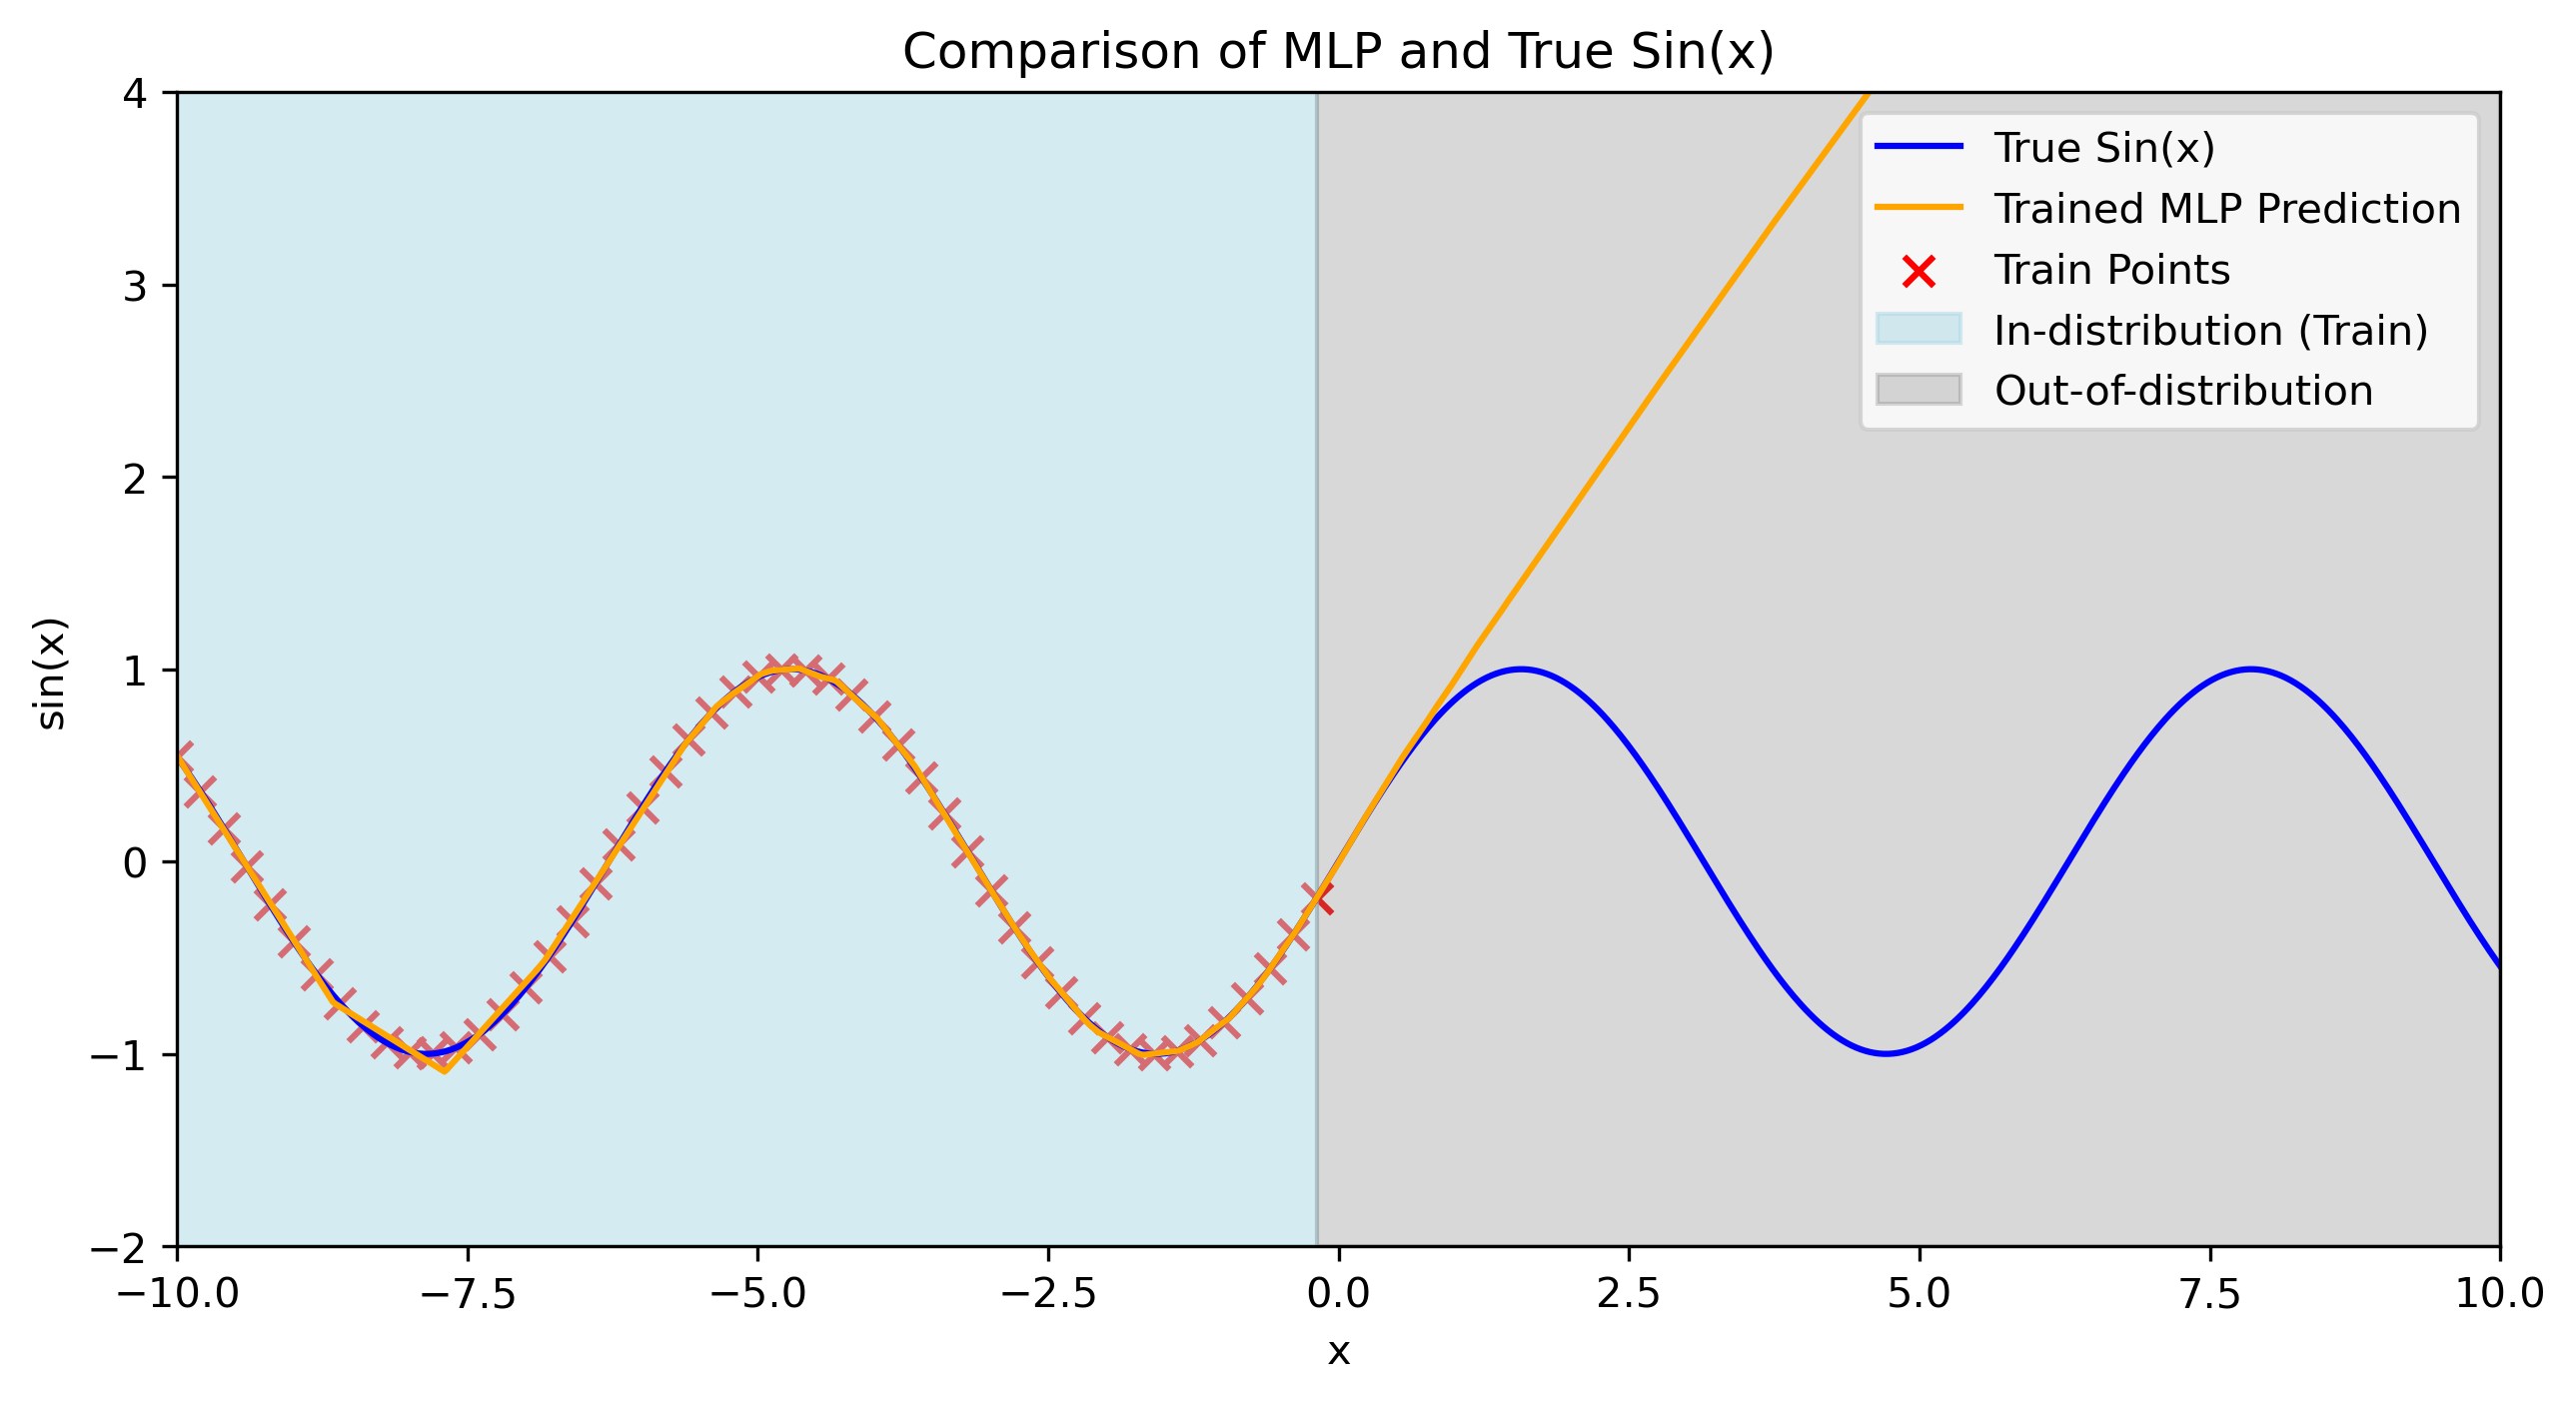
\includegraphics[width=0.9\textwidth]{figs/analytic_vs_nn_inductive_bias.png}
    \caption{Neural network prediction (one layer network with width 100 and ReLU activations)  versus symbolic model for sinusoidal dataset. The symbolic model is $y = sin(x)$.}
    \label{fig:nn_vs_sym_sin}
\end{figure}

\subsection{Symbolic Distillation Framework}
The general framework prescribed by the paper for symbolic distillation is as follows:
\begin{itemize}
    \item Design a neural network with an architecture that has a seperable internal structure and an inductive bias that is well suited to modelling the underlying problem.
    \item Train the model with regularisation techniques that encourage the network to learn a low-dimensional representation of the data.
    \item Replace a component of the neural network with a symbolic model that approximates the neural network's output.
    \item Retrain the neural network with the symbolic model as a component, and repeat the process until all components of the neural network have been replaced with low dimensional symbolic models.
\end{itemize}

% Why even add NNs - factorisation of the search space.
This framework may prompt the question: what is the necessity of employing neural networks initially? Why not directly utilize symbolic regression? The issue arises from the high dimensionality of modern datasets, which renders the application of symbolic regression, essentially a brute-force search over the space of all possible equations, computationally infeasible. To illustrate this point and the motivation behind this work, consider the problem of discovering a force law from a dataset of observed instantaneous accelerations of particles $\mathbf{a}_i \in \mathbb{R}^n$ and their positions $\mathbf{x}_i \in \mathbb{R}^n$. Assume a force law of the form $\mathbf{f}_{ij} = -k |\mathbf{x}_i - \mathbf{x}_j|$, with $\mathbf{a}_i = \frac{\mathbf{F}_i}{m_i}$, where $\mathbf{F}_i = \sum_j \mathbf{f}_{ij}$. To learn symbolic models for the acceleration $\textbf{p}(\textbf{x})$ and the pairwise force $\textbf{q}(\textbf{x})$, one can apply the inductive bias $\textbf{a}_i = \textbf{p}(\sum_j \textbf{q}(\textbf{x}_i, \textbf{x}_j))$. If the symbolic regression model needs to search $N$ equations to fit a given model, the search space scales as $O(N^2)$. However, if neural networks are first used to approximate the functions $\mathbf{p}(x)$ and $\mathbf{q}(x)$, and symbolic regression is subsequently applied to approximate these neural networks, the models can now be fit independently, reducing the search space to $O(N)$. If the dimensionality of the problem $n$ increases or the force law becomes more complex, the number of equations $N$ required to search also increases significantly. Therefore, this factorization of the search space is essential to make symbolic regression tractable for high-dimensional problems.
\subsection{Graph Neural Networks}
The work in the original paper and this report is primarily related to the class of problems which can be classed as interacting particle problems. This type of problem describes a very broad range of most problems encountered in physics. The graph neural network architecture applies a well suited inductive bias to these problems. This section will briefly describe the fundamental components of the graph neural network architecture and why it is well suited to interacting particle problems.

A graph neural network (GNN) is a specialised architecture designed to operate on graph data structures, where nodes represent particles and edges represent pairwise interactions between particles. In this context, each node has an associated feature vector encoding properties such as position, velocity, mass, and charge. The GNN operates through a scheme of message passing, involving two main components: the edge model ($\phi_e$) and the node model ($\phi_v$).
\paragraph*{Edge Model ($\phi_e$):}
   \begin{itemize}
       \item The edge model is applied to each edge in the graph.
       \item It takes as input the feature vectors of the two nodes connected by the edge.
       \item Formally, $\phi_e : \mathbb{R}^{d_v} \times \mathbb{R}^{d_v} \rightarrow \mathbb{R}^{d_e}$, where $d_v$ is the dimensionality of the node feature vectors, and $d_e$ is the dimensionality of the edge messages.
       \item The output of the edge model is called an edge message.
   \end{itemize}

\paragraph*{Node Model ($\phi_v$):}
   \begin{itemize}
       \item Once every edge has an associated edge message, the node model is applied to each node in the graph.
       \item It takes as input the feature vector of the node and the aggregated edge messages from all inbound edges.
       \item Aggregation is performed using a summation operator.
       \item Formally, $\phi_v : \mathbb{R}^{d_v} \times \mathbb{R}^{d_e} \rightarrow \mathbb{R}^{d_v'}$, where $d_v'$ is the dimensionality of the updated node feature vectors.
       \item The output of the node model is the updated node feature vector.
   \end{itemize}

This message-passing process is repeated for a number of layers, with the output of the final layer being the output of the graph neural network. The computational graph of the GNN is shown in Figure \ref{fig:gnn}, illustrating the interactions between nodes and edges through the edge and node models.

The graph neural network is an appropriate inductive bias for a variety of reason. Firstly, many important forces in physics are defined on pairs of particles, analogous to the message function of the Graph Networks. Further, the summation that aggregates messages is analogous to the calculation of the net force on a receiving particle. Finally, the node function is analogous to the application of Newton's second law: acceleration equals the net force (the summed message) divided by the mass of the receiving particle. Further, the graph neural network architecture is invariant under particle permutations, which is a desirable property for a model which represents interacting particle problems. 

It will be the edge and node models of the graph neural network that will be replaced by symbolic models in the symbolic distillation framework. The goal will be to recover the underlying force law used to generate the data.
\begin{figure}[H]
    \centering
    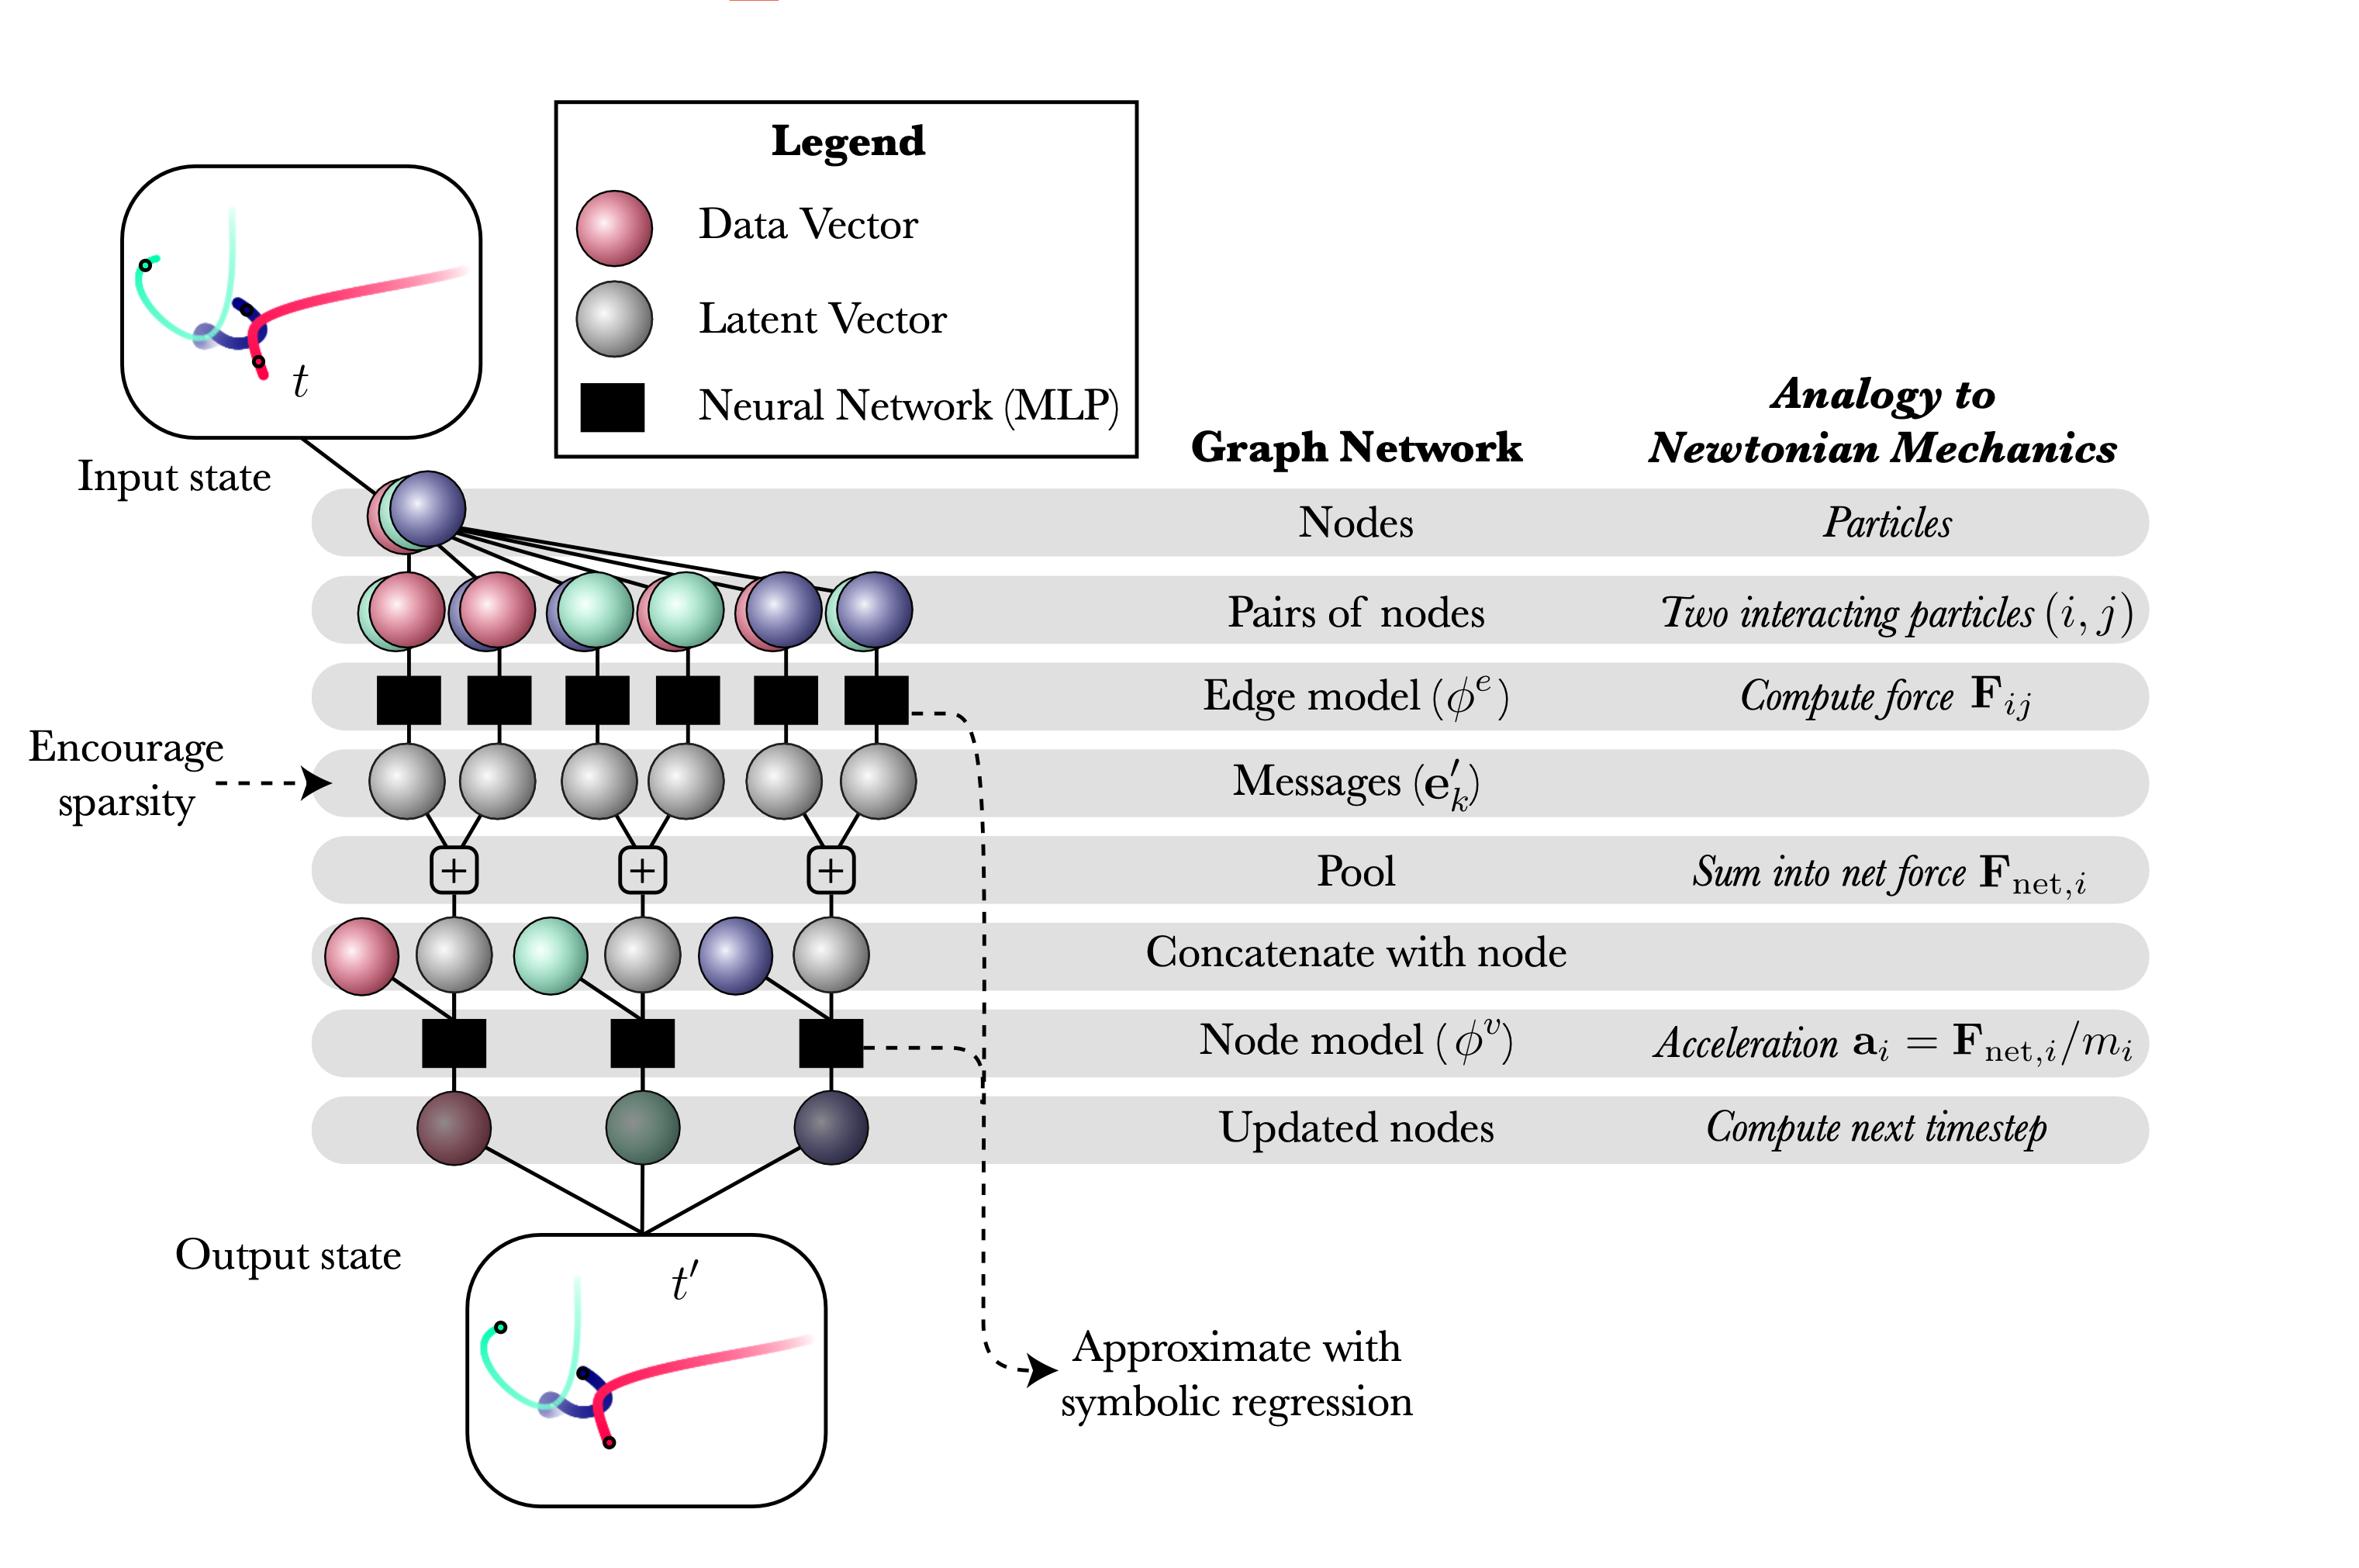
\includegraphics[width=0.9\textwidth]{figs/gnn_diagram.png}
    \caption{Computational graph of the graph neural network architecture. Diagram taken from Cranmer et al. \cite{cranmer2020discovering}}
    \label{fig:gnn}
\end{figure}
% Explain what they are and why they present the appropriate inductive bias for the problem.

% force law interacting particle problems - Fri
% Introduce the data briefly and the pipeline for the problem.
\section{Data}
This section will outline the datasets used in the experiments and the pipeline for the problem. The dataset consists of N-body particle simulations for a variety of force laws. From the original paper, the following force laws are investigated:
\begin{itemize}
    \item Spring: \(\textbf{f}_{ij} = -(|\textbf{r}_{ij} - 1|) \hat{\textbf{r}}_{ij}\)
    \item \(\frac{1}{r}\) Orbital force: \(\textbf{f}_{ij} = -\frac{m_i m_j\hat{\textbf{r}}_{ij}}{|\textbf{r}_{ij}|}\)
    \item \(\frac{1}{r^2}\) Orbital force: \(\textbf{f}_{ij} = -\frac{m_i m_j \hat{\textbf{r}}_{ij}}{|\textbf{r}_{ij}|^2}\)
    \item Charge: \(\textbf{f}_{ij} = -\frac{q_i q_j \hat{\textbf{r}}_{ij}}{|\textbf{r}_{ij}|^2}\)
\end{itemize}
Each force law was simulated in 2D and 3D, with 4 and 8 particles respectively. For each experiment, 10000 simulations were run in parallel for 500 time steps. This was split 3:1 to obtain the training and validation set. The test set was generated separately. The initial positions and velocities were randomly sampled from a normal distribution, the mass was sampled from a log normal distribution and the charge was drawn randomly from the set \(\{-1, 1\}\). 
% Original paper dataset size vs this one 
It is worth noting that the original paper ran each simulation for 1000 time steps, however, to avoid model training times becoming prohibitively long, the simulations were run for half the number of time steps. The step size varies for each simulation due to the differences in scale. It is: 0.005 for \( \frac{1}{r} \), 0.001 for \( \frac{1}{r^2} \), 0.01 for Spring, 0.001 for Charge. The code used to generate the simulations is available in the repository under the \texttt{simulations} directory. 
% Preprocessing
\subsection{Preprocessing}
Due to the nature of orbital and charge force laws, their dependence on \(r\) with a negative power can lead to exploding force values when particles are too close. This causes the data to vary over a scale too large for a neural network to learn effectively. To mitigate this, a small epsilon (\(10^{-2}\)) was added to the denominator, squashing \(r\) values into a more manageable range. Despite this, some experiments were found to have velocity distributions that still contaned extremely large outliers. To address this, a preprocessing step was introduced. The velocities and accelerations were pruned based on upper and lower percentile bounds. If any particle in a given timestep had a velocity or acceleration outside these bounds, the entire graph for that timestep was removed. This ensured that only timesteps where all particles had acceptable values were retained, improving data quality and consistency. Note, while this breaks the time continuity of the data, it is important to note that the data need not be continuous in time, as each time step defines a complete graph input to the neural network. The impact of this preprocessing step for the 2D Charge data in \ref{fig:distributions}. To see more detailed summary statistics showing the effect of this step, refer to the appendix.
\begin{figure}[H]
    \centering
    \begin{subfigure}{0.9\textwidth}
        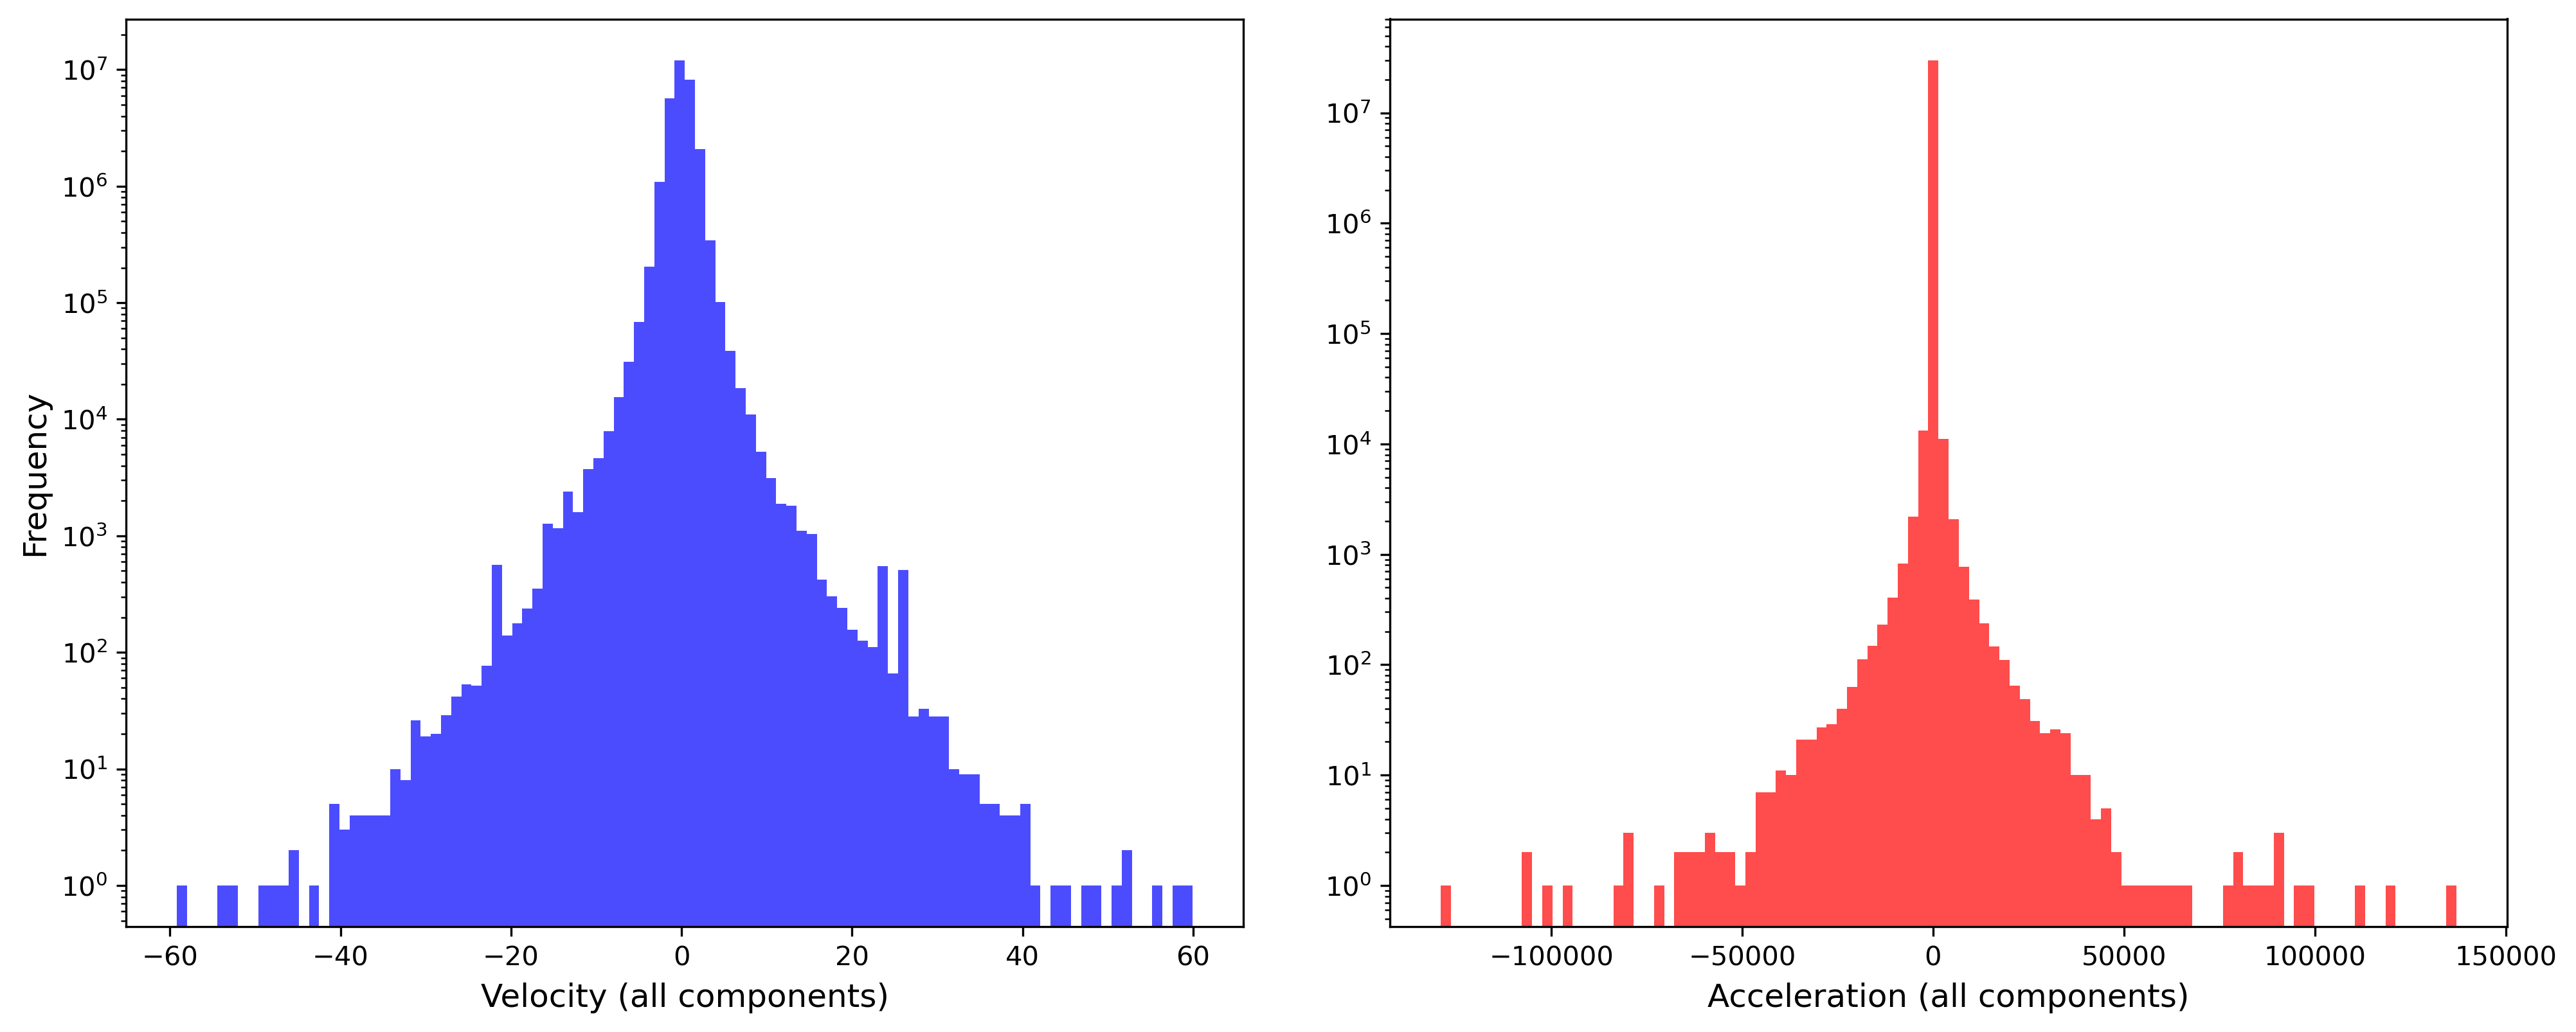
\includegraphics[width=\textwidth]{figs/charge_2_accel_vel_dist_unpruned.png}
        \caption{Charge 2D velocity distribution}
        \label{fig:charge_2_vel_dist_unpruned}
    \end{subfigure}
    \begin{subfigure}{0.9\textwidth}
        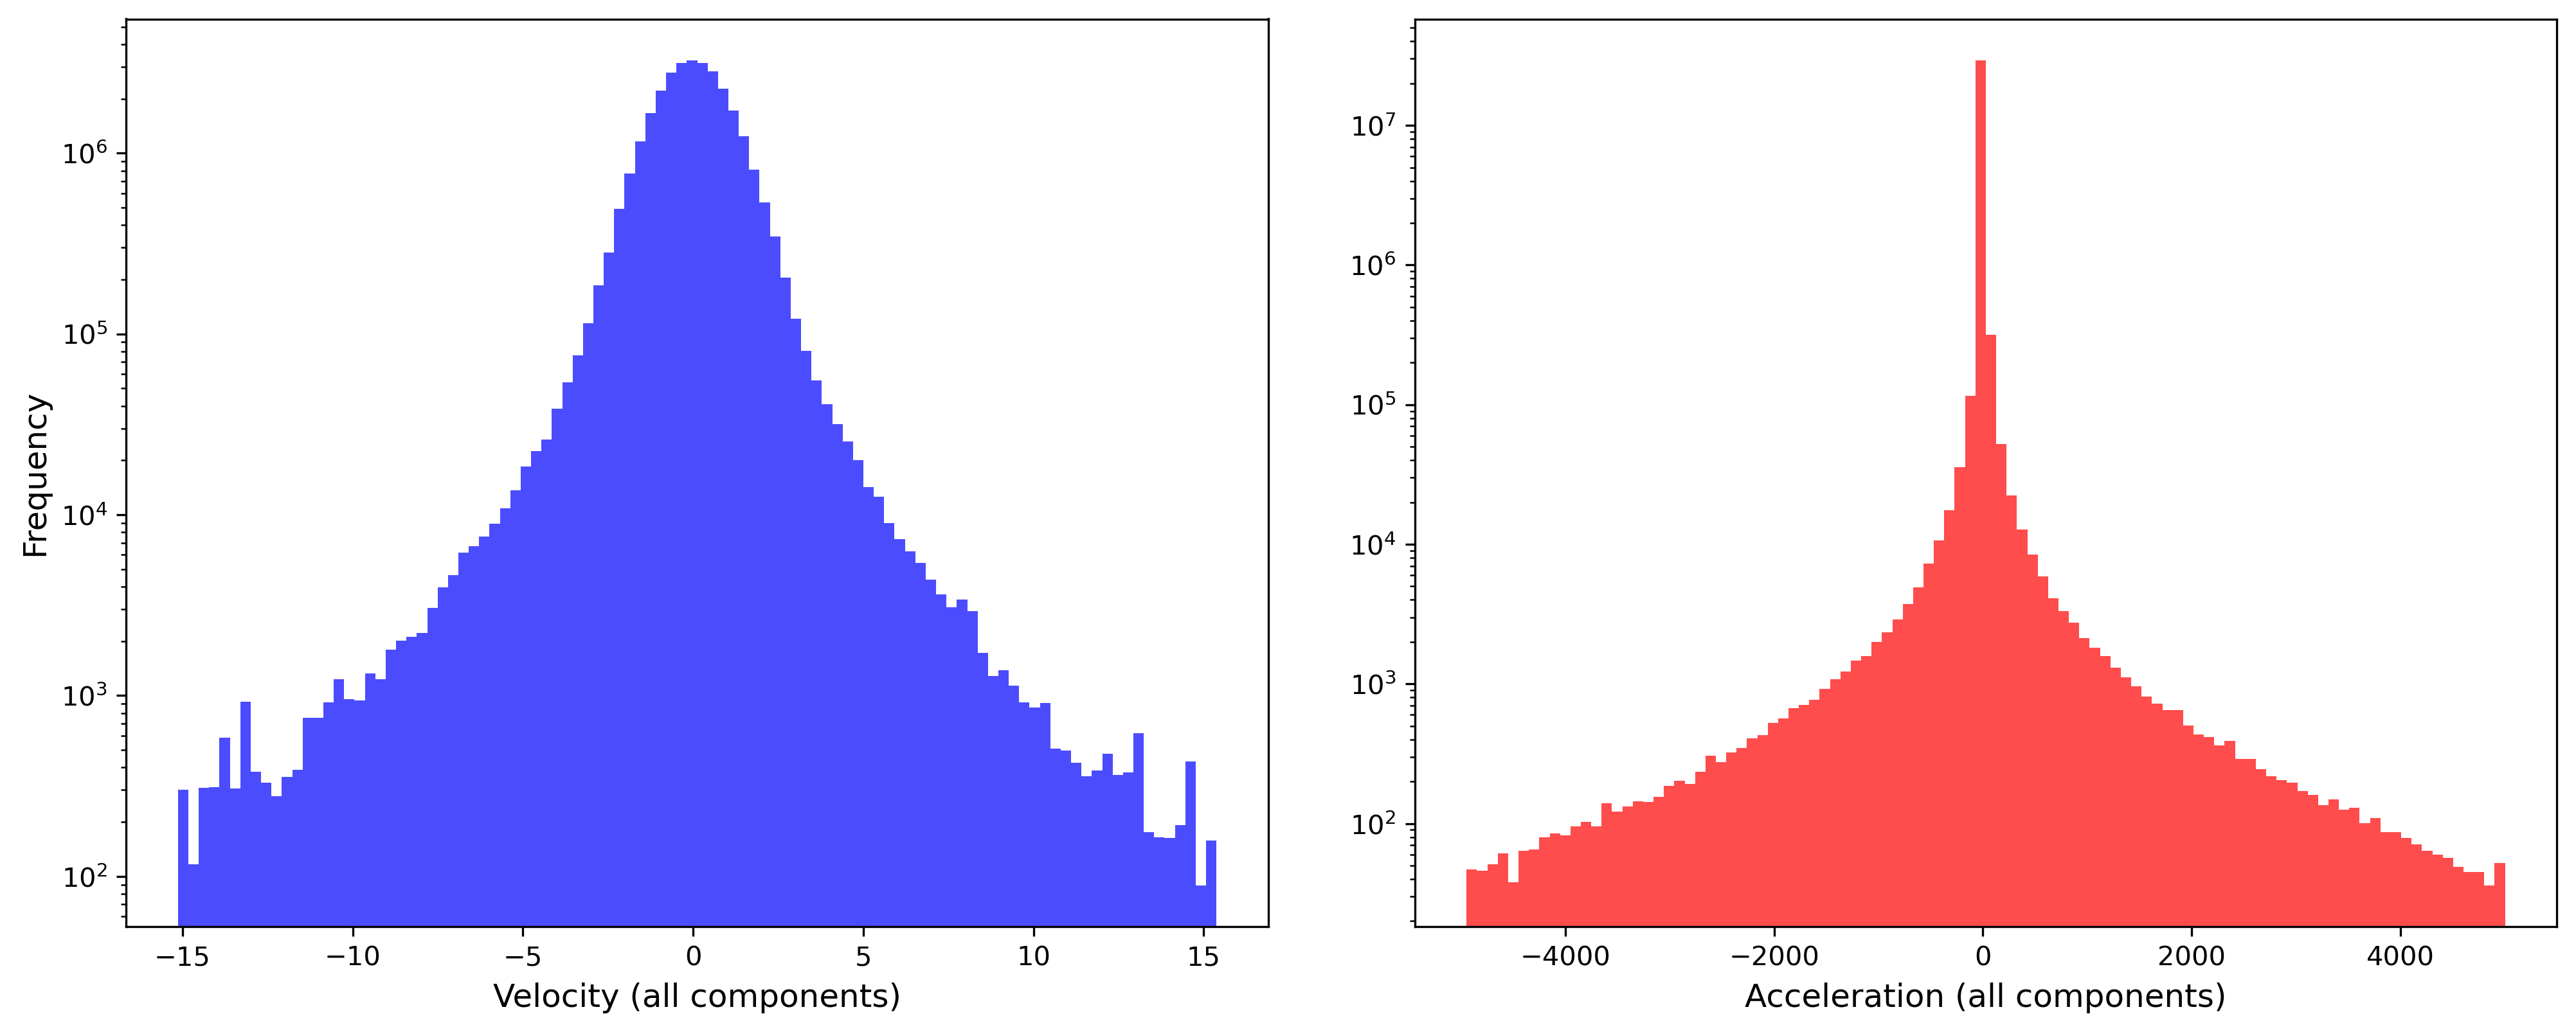
\includegraphics[width=\textwidth]{figs/charge_2_accel_vel_dist_pruned.png}
        \caption{Charge 2D velocity distribution (pruned)}
        \label{fig:charge_2_vel_dist_pruned}
    \end{subfigure}
    \caption{Velocity and acceleration distributions for Charge 2D data before and after preprocessing}
    \label{fig:distributions}
\end{figure}


\section{Method}
This section outlines the method used to train a graph neural network to predict instantaneous accelerations of particles.

\subsection{Training strategies}
This report investigates 4 of the training strategies outlined in the original paper. The training strategies are as follows: standard, KL, bottleneck and L1. 

\paragraph*{Standard Strategy}
The standard training strategy serves as the baseline case where the edge message dimensionality is 100 and the loss does not include any regularisation terms. Here the loss function is given by the mean absolute error between the predicted and true accelerations.

\paragraph*{KL Strategy}
The KL strategy involves sampling edge messages from a multivariate normal distribution as defined by the output of the edge model, which is now a 200-dimensional vector, with the first 100 dimensions representing the mean and the second 100 dimensions representing the log variance. Additionally, the average Kullback-Leibler divergence penalty over all edge messages, using a standard normal as the prior, is added to the loss. The weight of this term is set to \(1.0 \).

\paragraph*{L1 Strategy}
The L1 strategy is the same as the standard, except it now incorporates the L1 norm of the edge message as a regularisation term, averaged over all edge messages, in the loss. The weight of this term is set to \(1.0 \times 10^{-2}\).

\paragraph*{Bottleneck Strategy}
The bottleneck strategy is the same as the standard, however now aligns the dimensionality of the edge message with the dimensionality of the problem (2 or 3).

% Introduce the architecture of the model
\subsection{Model Architecture}
The architecture of the graph neural network (GNN) employed across various training strategies is consistent, except for variations in the output dimension of the edge model. The GNN comprises two multi-layer perceptrons (MLPs): the edge model and the node model.

\paragraph*{Edge Model} This model consists of two hidden layers, each with 300 units and ReLU activation functions. It takes as input the concatenated feature vectors from a pair of nodes connected by an edge in the graph. Each input vector is a $(2d+2)$-dimensional representation of position, velocity, mass, and charge, where $d$ represents the problem's dimensionality (2 or 3). The output dimension of the edge model varies depending on the training strategy.

\paragraph*{Node Model} Mirroring the edge model in structure, the node model takes as input the summed edge messages from all inbound edges to a given node, concatenated with the node's feature vector. Its output is a vector of dimension 2 or 3, corresponding to the predicted instantaneous acceleration of the node.

\subsection{Model Training}
The network is trained over 100 epochs using the Adam optimizer with an initial learning rate of \(0.001\) and weight decay set to \(1.0 \times 10^{-8}\). It is worth noting that this is half the number of epochs used in the original paper. The learning rate is modulated by the 1cycle learning rate policy \cite{smith2018superconvergence}, which increases the learning rate to a peak of \(0.001\) before gradually decreasing it by a factor of \(100,000\), adhering to a pre-defined schedule. Random translation is used as a form of data augmentation to improve the model's generalisation capabilities. The model is trained on a single NVIDIA A100 GPU.

\subsection{Symbolic Regression of the Network}
% Explain how the sybolic regressor was fit - used less operations than the paper to make it easier to reduce the search space
After training the model end to end, the edge and node model are symbolically distilled using the \texttt{PySR} package \cite{cranmer2023interpretable}. PySR's internal search algorithm is a multi-population evolutionary algorithm, which consists of a unique evolve-simplify-optimise loop, designed for optimisation of unknown scalar constants in newly-discovered empirical expressions. 100 populations were used and evolved for 100 iterations. The random state was set to 42. The operators considered in the fitting process are $ +, -, \times , /$ as well as real constants. Note, this is a subset of the operators used in the original paper when fitting for symbolic models. This was done to reduce the search space and quickly check that the symbolic distillation framework was working as expected.

\subsubsection{Model Selection Criteria}
The best symbolic model is selected by evaluating the mean absolute error (MAE) and the complexity of the model. The complexity is scored by counting the number of occurrences of each operator, constant, and input variable. PySR outputs several equations at each complexity level. The chosen formula is one that maximises the fractional drop in MAE over an increase in complexity from the next best model.

\subsubsection{Symbolic Distillation of the Edge Model}
To symbolically distil the edge model, its inputs and outputs are recorded over the test set. The input comprises the concatenated feature vectors of two nodes connected by an edge, including the position, velocity, mass, and charge of each node ($(m_1, m_2, q_1, q_2, x_1, x_2, \ldots)$). Given that force laws depend on the relative positions of the nodes, To simplify, the positions are converted to $\Delta x = x_2 - x_1$ for displacement, similarly for $y$ (and $z$ in 3D), and $r = \sqrt{\Delta x^2 + \Delta y^2 + (\Delta z^2)}$ for distance. This array of $(m_1, m_2, q_1, q_2, \Delta x, \Delta y, (\Delta z), r)$ comprises as the input to the symbolic model. Next, the $d$ most significant components of the corresponding edge message are selected as the output labels for the symbolic regression model. Significance here is defined by the components of the edge message with the highest standard deviation across the samples, where $d$ is the dimensionality (2 or 3). In the bottleneck strategy, the edge message is already of the correct dimensionality, so no further processing is needed. In the original paper, 5000 samples are collected from the data in the test set, however in this analysis 1000 samples are used to reduce the computational cost of the symbolic regression.

\subsubsection{Symbolic Distillation of the Node Model}
The symbolic distillation of the node model is similar to that of the edge model. The input to the symbolic model is the node's feature vector, which includes the position, velocity, mass, and charge of the node ($(m_1, q_1, x_1, \ldots)$), and the aggregated inbound edge messages. The aggregation is not performed over the full 100 dimensions of the edge message, but rather the $d$ most significant components, where $d$ is the dimensionality of the problem (2 or 3). The output of the symbolic model is the predicted instantaneous acceleration of the node. In the original paper, 5000 samples are collected from the data in the test set, however in this analysis 1000 samples are used to reduce the computational cost of the symbolic regression.


\subsection{Evaluation metrics}
To evaluate model performance, the mean absolute error (MAE) between the predicted and true accelerations is calculated over the test set. This metric assesses the predictive capabilities of the trained model. Additionally, the standard deviation of the top 15 edge messages is computed to evaluate the compactness of the learnt representations. This metric indicates whether the training resulted in a model that correctly captured the problem's dimensionality. The $R^2$ metric between the significant edge message components and a linear transformation of the true pairwise force is also calculated. The specific linear transformation is found through a minimisation the mean squared error (MSE) between observed message components and those predicted by a linear combination of force components. This is implemented through using the \texttt{minimize} function from the \texttt{scipy.optimize} module, employing the Powell method. The optimisation only considers the MSE errors within the 90th percentile of their absolute values, thereby reducing the influence of outliers. This is the same method used in the original paper. The appendix of the original paper provides a mathematical argument for why the model would learn a linear transformation of the pairwise force. Finally, the trained model is evaluated through symbolically regressing its edge and node models and checking how many components yield a linear transformation of the true pairwise force and newtons second law respectively.

\section{Results}
% Check that if while the edge model might not always be pairwise force, the node model should always just be returning aggr or a scaled version since nns like to learn identity funcs. Cool talking point

\subsection{Model Performance}
The first set of results to be presented are the mean absolute error (MAE) loss on the test set for each simulation. The results are presented in Table \ref{tab:mae_table_with_std}. The best values across different training strategies are shown in bold. Values are also highlighted in bold when their confidence intervals overlap with the lowest MAE value for a given simulation. Two conclusions can be arrived at from this set of results. Firstly, that the KL is the worst by a significant margin as it always has an MAE and standard deviation value that is atleast an order of magnitude larger than those given by the other strategies. The second observation is that while the bottleneck strategy gives the best performance in five out of eight simulations, the margin by which it leads is minimal. This suggests that the other strategies exhibit comparable efficacy in optimising for MAE, with no clear dominant strategy across the board.
\begin{table}[H]
    \centering
    \begin{tabular}{lcccc}
    \hline
    Sim & Standard & Bottleneck & L$_1$ & KL \\
    \hline
    Charge-3 & \textbf{0.110} $\pm$ 0.015 & \textbf{0.140} $\pm$ 0.022 & 0.157 $\pm$ 0.019 & 3.325 $\pm$ 0.168 \\
    Charge-2 & \textbf{0.466} $\pm$ 0.211 & \textbf{0.462} $\pm$ 0.186 & \textbf{0.483} $\pm$ 0.178 & 3.267 $\pm$ 0.417 \\
    r$^{-2}$-3 & \textbf{0.1753} $\pm$ 0.042 & \textbf{0.1746} $\pm$ 0.043 & \textbf{0.2128} $\pm$ 0.050 & 3.8264 $\pm$ 0.264 \\
    r$^{-2}$-2 & \textbf{0.475} $\pm$ 0.169 & \textbf{0.461} $\pm$ 0.167 & \textbf{0.450} $\pm$ 0.142 & 4.0380 $\pm$ 0.557 \\
    r$^{-1}$-3 & 0.0283 $\pm$ 0.003 & \textbf{0.0261} $\pm$ 0.003 & 0.0408 $\pm$ 0.004 & 3.251 $\pm$ 0.101 \\
    r$^{-1}$-2 & 0.0254 $\pm$ 0.005 & \textbf{0.0238} $\pm$ 0.005 & 0.0326 $\pm$ 0.004 & 2.3365 $\pm$ 0.147 \\
    Spring-3 & \textbf{0.0566} $\pm$ 0.003 & 0.0595 $\pm$ 0.003 & 0.0728 $\pm$ 0.004 & 2.6839 $\pm$ 0.057 \\
    Spring-2 & 0.0200 $\pm$ 0.001 & \textbf{0.0182} $\pm$ 0.001 & 0.0249 $\pm$ 0.001 & 1.7455 $\pm$ 0.066 \\
    \hline
    \end{tabular}
    \caption{Mean Absolute Error (MAE) loss on the test set, presented as mean $\pm$ standard deviation. The best values across different training strategies are shown in bold. Values are highlighted in bold when their confidence intervals overlap with the lowest MAE value for a given simulation.}
    \label{tab:mae_table_with_std}
    \end{table}

For comparison, the MAE values for the original paper are presented in Table \ref{tab:mae_table_original}. Unfortunately the original paper does not provide the spread of the MAE values, so it is not possible to compare the standard deviations of the MAE values. However, the original paper also follows the general trend of the standard, bottleneck and L1 performing similarly, with the KL strategy performing significantly worse. However, as a whole, the MAE values in this report are lower than those in the original paper, this is discussed in the next section and is likely due to the preprocessing steps taken to improve data quality that were not present in the original paper. These results refute the claim made by the original paper that the L$_1$ strategy performs better than the bottleneck strategy. The findings in this report, and indeed in those presented in the original paper, suggest that the bottleneck strategy, standard and L$_1$ strategies are comparable in terms of their ability to optimise for MAE, there is no clear dominant strategy across the board.

\begin{table}[H]
    \centering
    \begin{tabular}{lcccc}
    \hline
    Sim & Standard & Bottleneck & L$_1$ & KL \\
    \hline
    Charge-3 & 1.2  & 0.99  & \textbf{0.94}  & 4.2  \\
    Charge-2 & \textbf{49}  & 50  & 52  & 60  \\
    r$^{-2}$-3 & 4.0 & 3.6  & \textbf{3.4} & 9.8  \\
    r$^{-2}$-2 & 1.6  & 1.6  & \textbf{1.2}  & 9.3  \\
    r$^{-1}$-3 & 0.051 & \textbf{0.050}  & 0.055 & 3.5   \\
    r$^{-1}$-2 & 0.077  & \textbf{0.069}  & 0.079  & 3.5   \\
    Spring-3 & 0.11  & 0.11  & \textbf{0.090}  & 3.8  \\
    Spring-2 & 0.047  & 0.046  & \textbf{0.045}  & 1.7  \\
    \hline
    \end{tabular}
    \caption{Mean Absolute Error (MAE) loss on the test set \textbf{in the original paper}. The best values across different training strategies are shown in bold}
    \label{tab:mae_table_original}
    \end{table}
\subsection{Edge Message $R^2$}
The next set of results presented are the $R^2$ values between significant edge message components and the linearly transformed true pairwise forces, averaged across all components. The results are presented in Table \ref{tab:R2}. For comparison, the $R^2$ values for the original paper are presented in Table \ref{tab:R2_original}. Example scatter plots of the edge message components against the linear transformation of the pairwise force for the different strategies of the spring 2D simulation are shown in Figure \ref{fig:scatter_plots}. It is clear that the R$_{2}$ values obtained are much lower for the bottleneck strategy and L$_{1}$ strategy which get almost perfect values in the original paper. The standard strategy in this report is found to have a significantly different value than that in the original paper which finds that in all simulations, it is very close to 0. These results are investigated in the discussion section.
    \begin{table}[H]
        \centering
        \begin{tabular}{lcccc}
        \hline
        Sim & Standard & Bottleneck & L$_1$ & KL \\
        \hline
        Charge-3 & 0.429 \textbf{(0.990)} & 0.817 (0.788) & 0.683 (0.897) & 0.251 (0.472) \\
        Charge-2 & 0.006 (0.050) & 0.700 \textbf{(0.897)} & 0.006 (0.055) & 0.381 (0.431)\\
        r$^{-2}$-3 & 0.502 (0.955) & 0.518 \textbf{(0.998)} & 0.505 (0.979) & 0.323 (0.564) \\
        r$^{-2}$-2 & 0.001 (0.397) & 0.411 \textbf{(0.985)} & 0.181 (0.528) & 0.291 (0.426) \\
        r$^{-1}$-3 & 0.402 \textbf{(0.999)} & 0.403 \textbf{(0.999)} & 0.364 (0.904) & 0.333 (0.859)\\
        r$^{-1}$-2 & 0.314 (0.962) & 0.324 \textbf{(0.994)} & 0.324 \textbf{(0.994)} & 0.250 (0.835) \\
        Spring-3 & 0.430 \textbf{(1.000)}& 0.430 \textbf{(1.000)} & 0.990 (0.438) & 0.918 (0.532)\\
        Spring-2 & 0.422 (0.999) & 0.999 (0.431) & \textbf{1.000} (0.430) & 0.768 (0.640) \\

        \hline
        \end{tabular}
        \caption{$R^2$ metric between the significant edge message components and a linear transformation of the true pairwise force (and pairwise acceleration shown in brackets). Best value across training strategy shown in bold (for either acceleration or force).}
        \label{tab:R2}
    \end{table}
    \begin{table}[H]
        \centering
        \begin{tabular}{lcccc}
        \hline
        Sim & Standard & Bottleneck & L$_1$ & KL \\
        \hline
        Charge-3 & 0.013 & \textbf{0.980} & 0.002 & 0.425 \\
        Charge-2 & 0.016 & \textbf{0.947} & 0.004 & 0.185 \\
        r$^{-2}$-3 & 0.002 & \textbf{0.994} & 0.977 & 0.214 \\
        r$^{-2}$-2 & 0.004 & 0.993 & \textbf{0.990} & 0.770 \\
        r$^{-1}$-3 & 0.000 & \textbf{1.000} & \textbf{1.000} & 0.332 \\
        r$^{-1}$-2 & 0.000 & \textbf{1.000} & \textbf{1.000} & 0.796 \\
        Spring-3 & 0.036 & 0.995 & \textbf{1.000} & 0.214 \\
        Spring-2 & 0.032 & \textbf{1.000} & \textbf{1.000} & 0.883 \\
        \hline
        \end{tabular}
        \caption{$R^2$ metric between the significant edge message components and a linear transformation of the true pairwise force \textbf{in the original paper}. Best value across training strategy shown in bold.}
        \label{tab:R2_original}
    \end{table}


    \begin{figure}[H]
        \centering
        \begin{subfigure}{0.45\textwidth}
            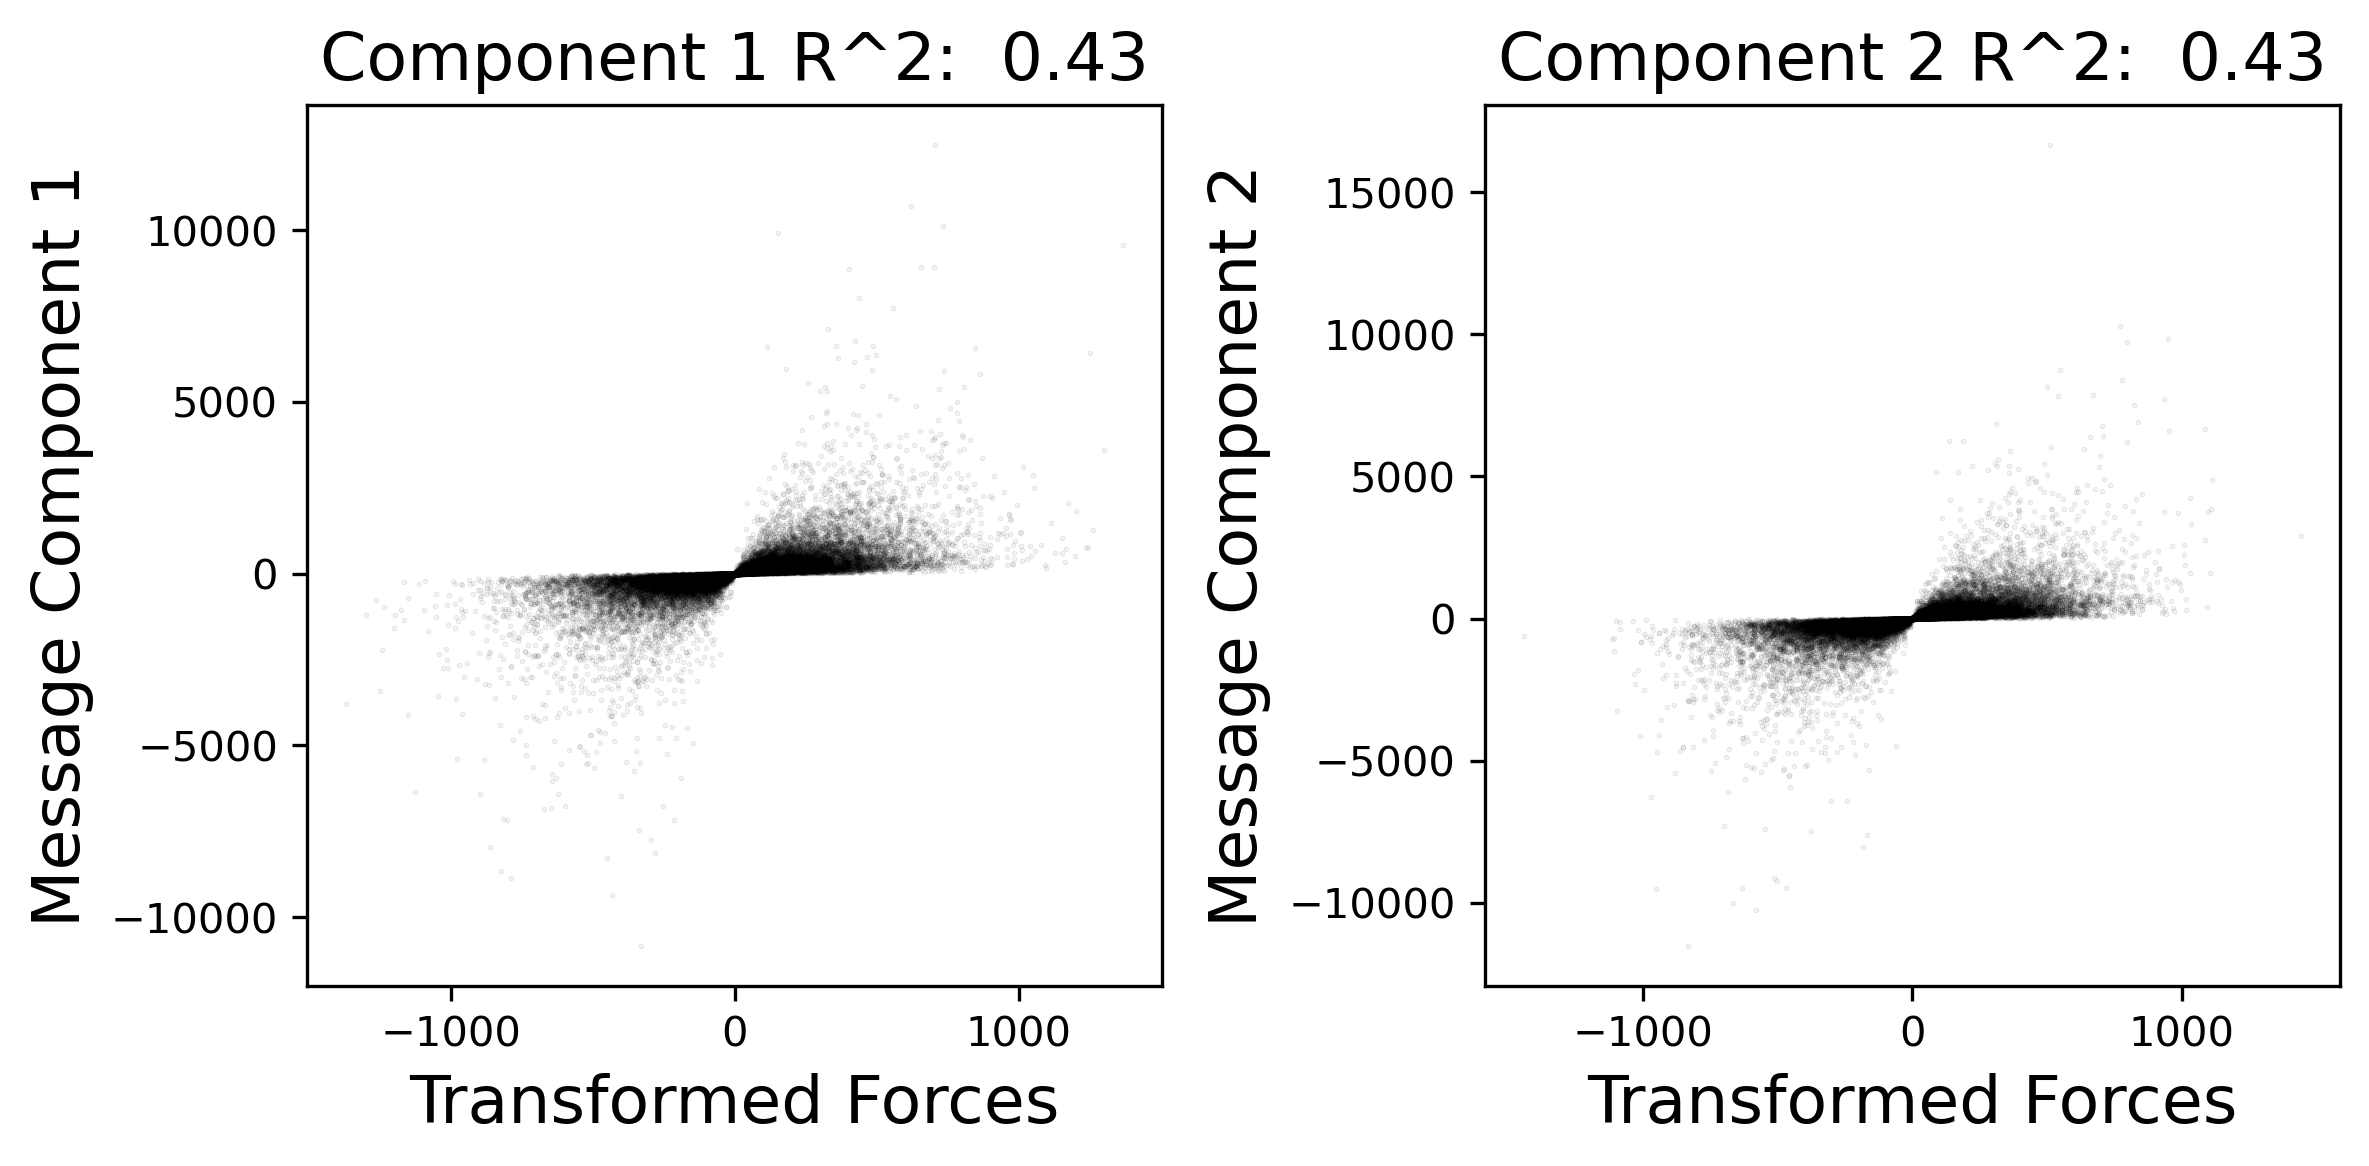
\includegraphics[width=\textwidth]{figs/spring_2d_standard_r2.png}
            \caption{Spring 2D, Standard}
        \end{subfigure}
        \begin{subfigure}{0.45\textwidth}
            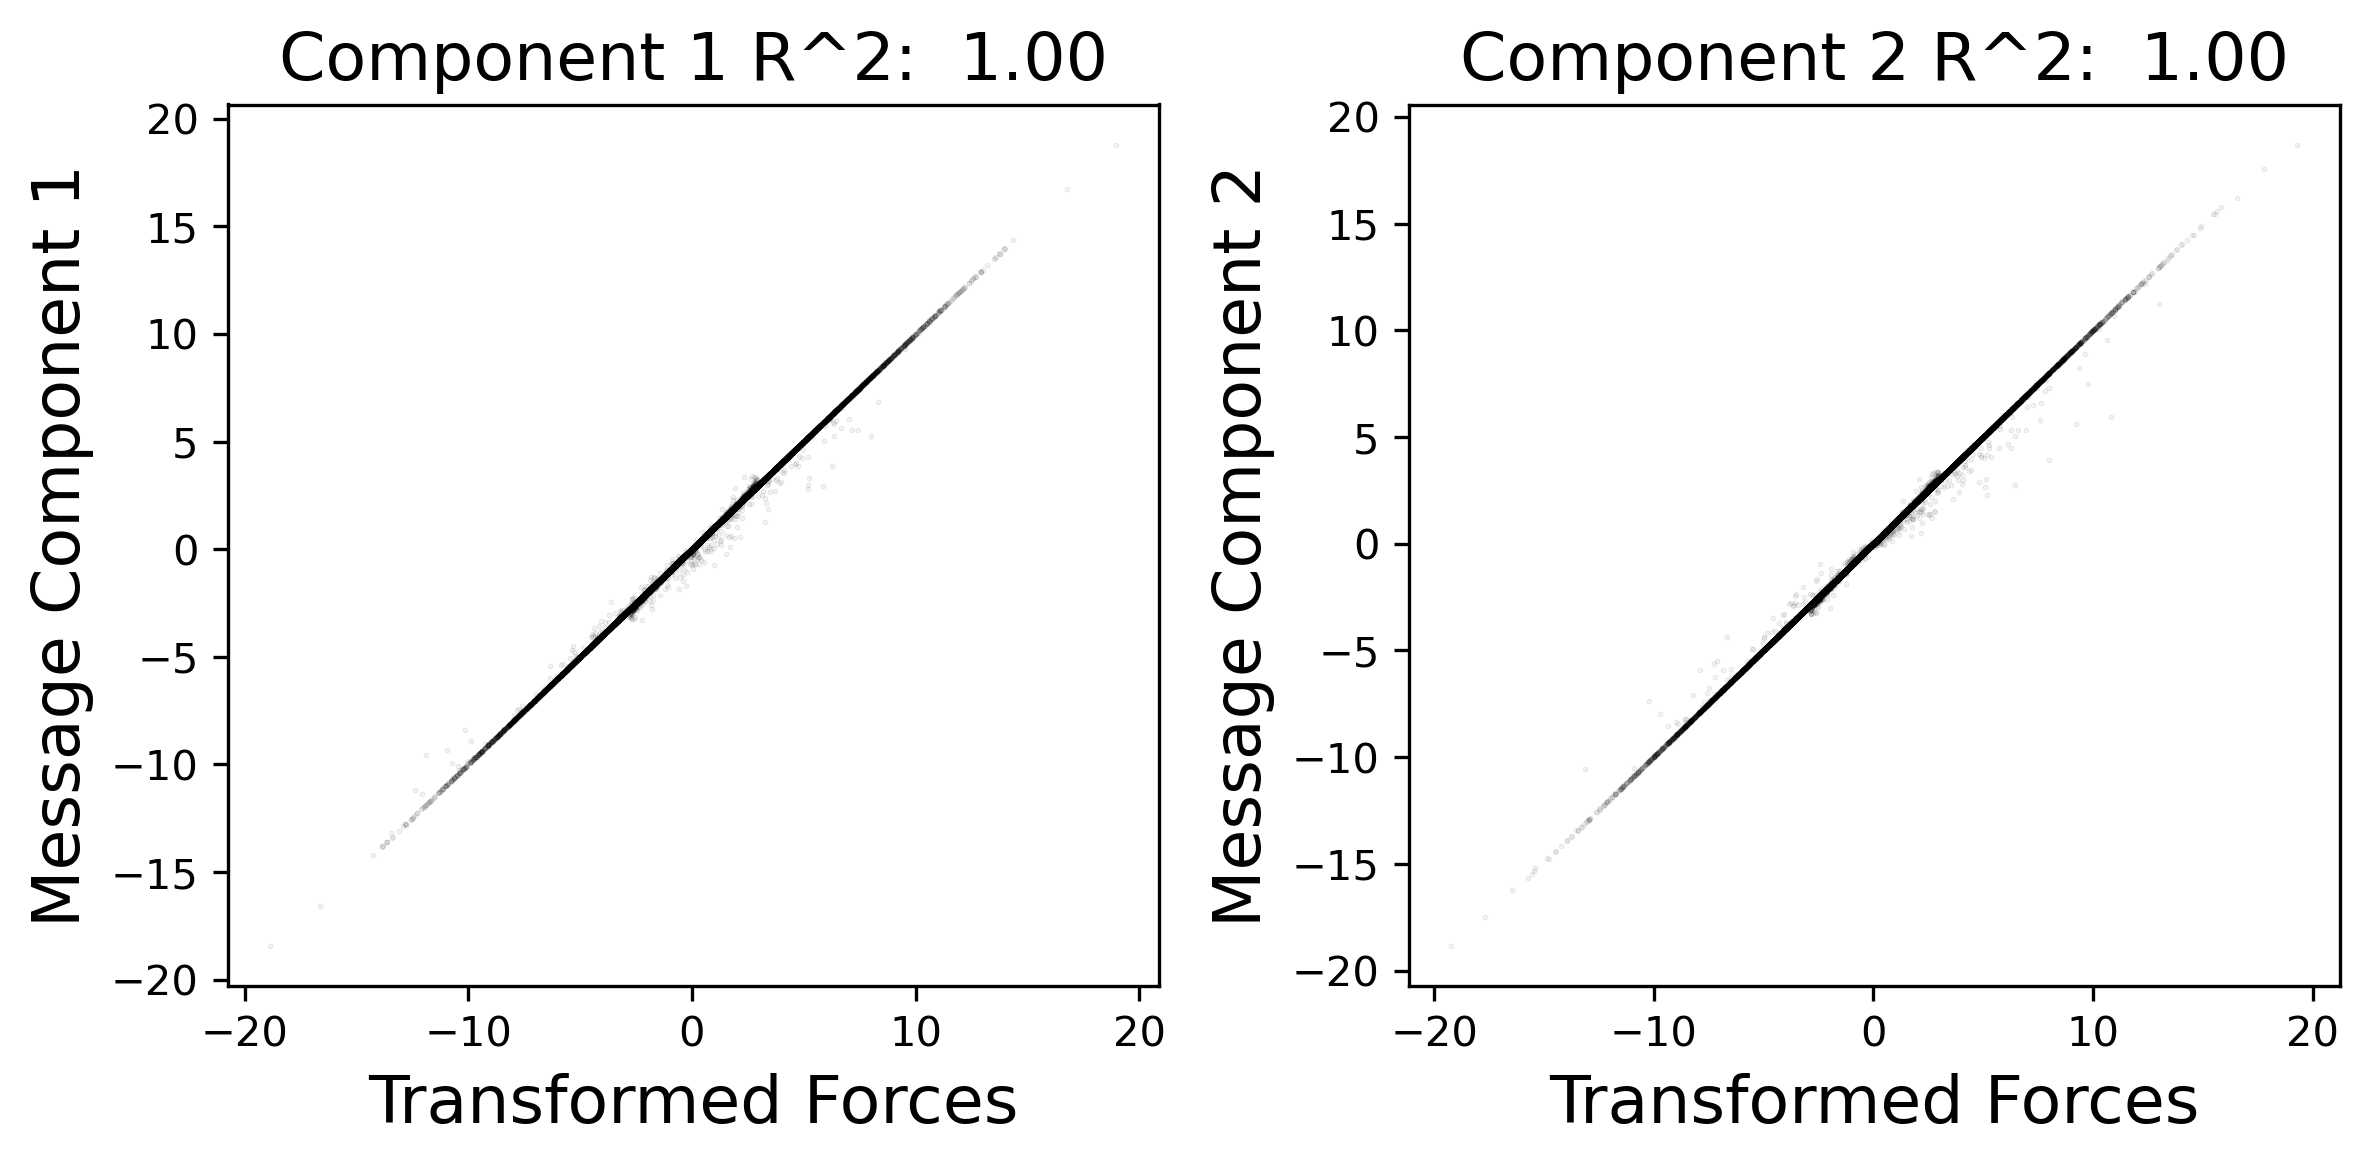
\includegraphics[width=\textwidth]{figs/spring_2d_bottleneck_r2.png}
            \caption{Spring 2D, Bottleneck}
        \end{subfigure}
        
        \begin{subfigure}{0.45\textwidth}
            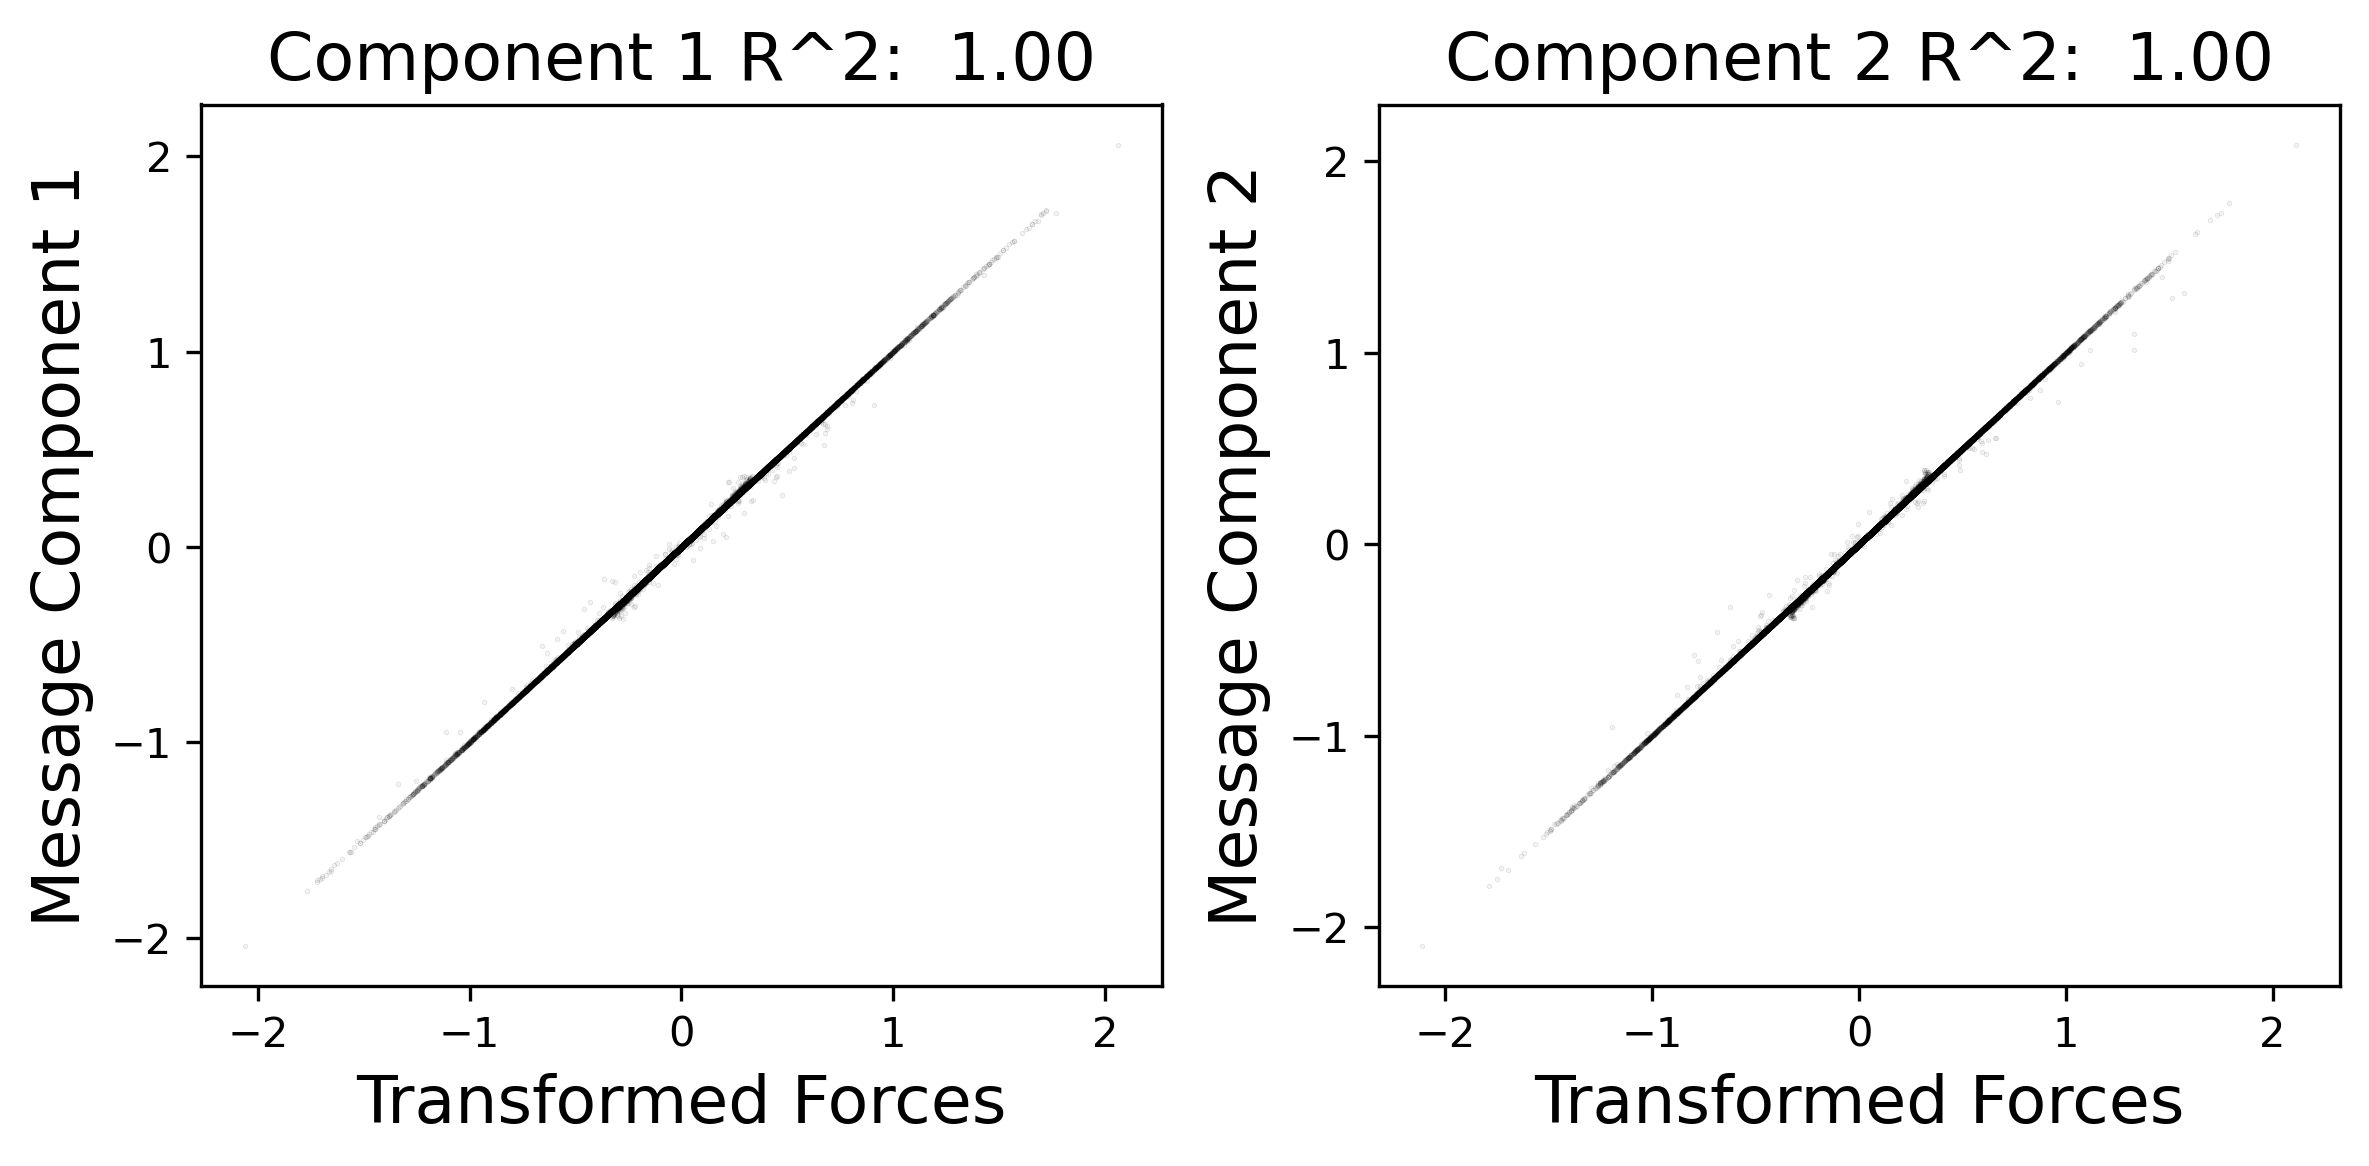
\includegraphics[width=\textwidth]{figs/spring_2d_l1_r2.png}
            \caption{Spring 2D, L$_1$}
        \end{subfigure}
        \begin{subfigure}{0.45\textwidth}
            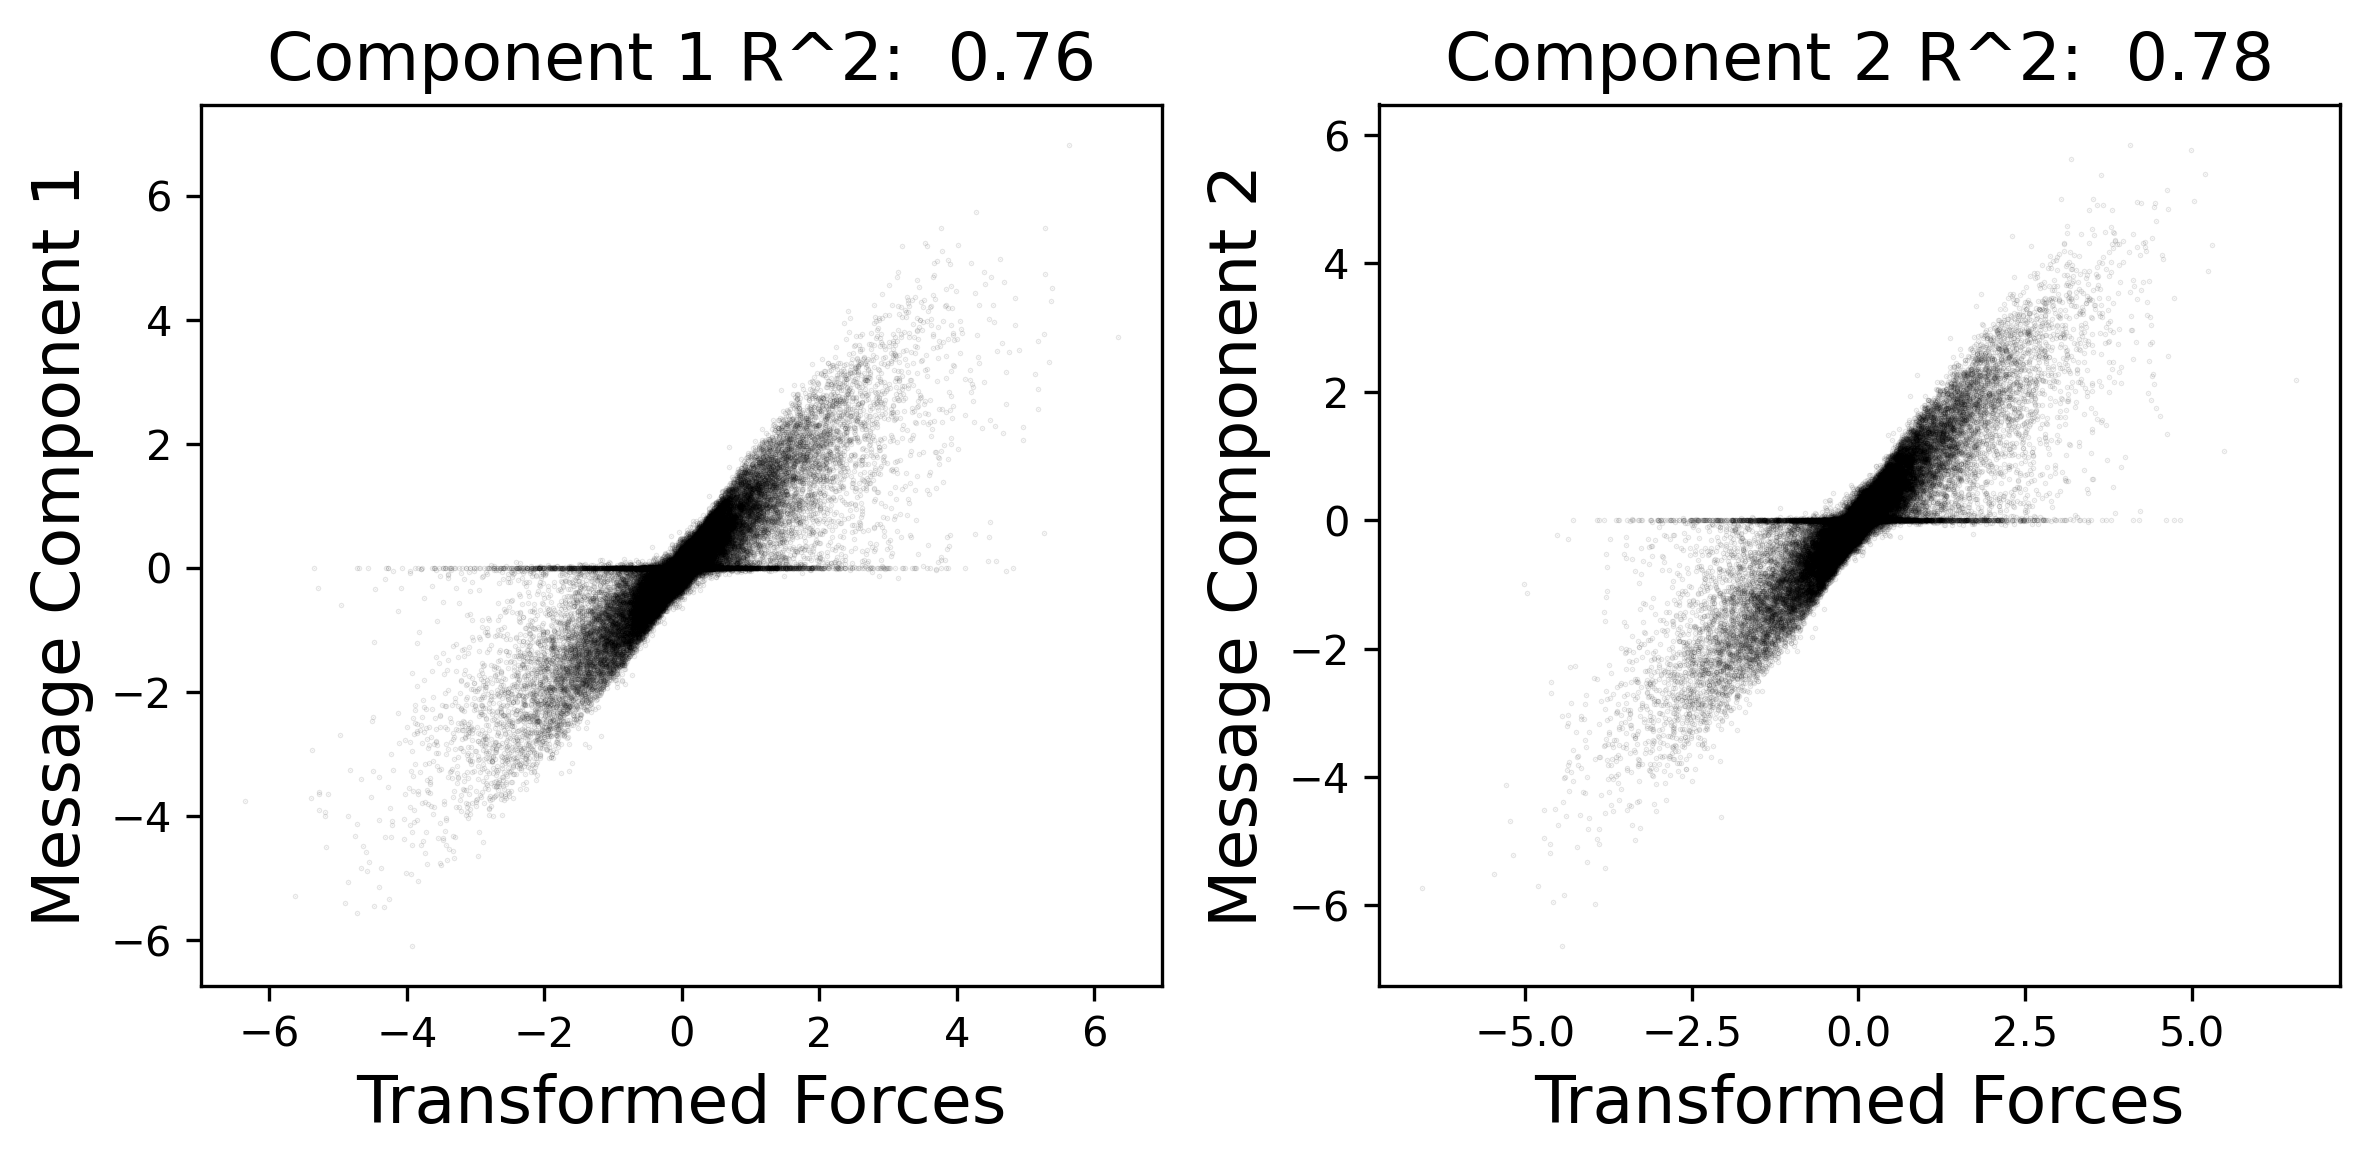
\includegraphics[width=\textwidth]{figs/spring_2d_kl_r2.png}
            \caption{Spring 2D, KL}
        \end{subfigure}
        \caption{Scatter plots of the edge message components against the linear transformation of the pairwise force for the different strategies of the spring 2D simulation.}
        \label{fig:scatter_plots}
    \end{figure}
    \subsection{Edge Message Sparsity}
    Next, to investigate the sparsity of the edge messages under the different training strategies, the percentage of total edge message variance across all components explained by the top $d$ components, where $d$ is the dimensionality of the problem, is calculated. The results are presented in Table \ref{tab:scarcity}. The KL and L$_1$ strategies consistently outperform the standard strategy. This suggests that the KL and L$_1$ strategies are more effective than the baseline at promoting sparsity in the edge messages. Note, the bottleneck strategy will always have, by definition, 100\% of the edge message variance explained by the top $d$ components.
    \begin{table}[H]
        \centering
        \begin{tabular}{lcccc}
        \hline
        Sim & Standard & Bottleneck & L$_1$ & KL \\
        \hline
        Charge-3 & 0.404 & 1.000 & 0.474 & 0.550 \\
        Charge-2 & 0.180 & 1.000 & 0.263 & 0.667 \\
        r$^{-2}$-3 & 0.583 & 1.000 & 0.795 & 0.925 \\
        r$^{-2}$-2 & 0.374 & 1.000 & 0.525 & 0.712 \\
        r$^{-1}$-3 & 0.877 & 1.000 & 0.743 & 0.719 \\
        r$^{-1}$-2 & 0.591 & 1.000 & 0.925 & 0.990 \\
        Spring-3 & 0.889 & 1.000 & 0.999  & 0.993 \\
        Spring-2 & 0.737 & 1.000 & 1.000 & 0.989 \\
        \hline
        \end{tabular}
        \caption{Percent of total edge message variance across all components explained by the top $d$ components, where $d$ is the dimensionality of the problem.}
        \label{tab:scarcity}
    \end{table}

\subsection{Symbolic Reconstructions}
The next set of results relate to the symbolic distillation of the edge and node models. The edge and node models are distilled seperately using the method outlined. The edge model's distillation should yield an expression which is approximately analogous to a linear transformation of the true force, whereas the node model's distillation should yield an expression which resembles Newtons second law.
\begin{table}[H]
        \centering
        \begin{tabular}{lcccc}
        \hline
        Sim & Standard & Bottleneck & L$_1$ & KL \\
        \hline
        Charge-3 & \textbf{3/3} & \textbf{3/3} & 0/3 & 0/3 \\
        Charge-2 & 0/2 & \textbf{2/2} & 1/2 & 0/2 \\
        r$^{-2}$-3 & 1/3 & \textbf{3/3} & \textbf{3/3} & 0/3 \\
        r$^{-2}$-2 & 0/2 & \textbf{2/2} & 0/2 & 1/2 \\
        r$^{-1}$-3 & \textbf{3/3} & \textbf{3/3} & 2/3 & \textbf{3/3} \\
        r$^{-1}$-2 & 0/2 & \textbf{2/2} & \textbf{2/2} & \textbf{2/2} \\
        Spring-3 & 0/3 & 2/3 & 2/3  & 0/3 \\
        Spring-2 & 1/2 & \textbf{2/2} & \textbf{2/2} & 0/2 \\
        \hline
        \end{tabular}
        \caption{Successful reconstructions of the pairwise force (or acceleration) after symbolically regressing the $d$ significant components of edge model, where $d$ is the dimensionality of the problem. Experiments where all components are successfully reconstructed are highlighted in bold.}
        \label{tab:sr_edge_model_table}
    \end{table}
From the results obtained, it is clear that the bottleneck strategy consistently outperforms the other strategies in the symbolic distillation of the edge model, the L$_1$ strategy is the next most successful, followed by the standard strategy and the KL strategy.

\paragraph*{Example successful reconstructions} of recovering the pairwise force (or acceleration) after symbolically regressing the edge model.
    \begin{itemize}
        \item
        Spring 2d, L$_1$ (expect $\phi^{e}_i \approx \mathbf{a} \cdot (1-\frac{1}{r}) \mathbf{\Delta {r}} + b$):
        $$
        \phi^{e}_1 = (-0.291 + \frac{0.287}{r})(\Delta x - 0.986 \Delta y) + 0.00118
        $$
        \item 
        r$^{-1}$ 2d, KL (expect $\phi^{e}_i \approx \mathbf{a} \cdot \frac{m_1 m_2}{r^2} \mathbf{\Delta r} + b$):
        $$\phi^{e}_2 = -\frac{0.273m_2(\Delta x + \Delta y)}{r^2}$$
        \item 
        r$^{-2}$ 3d, bottleneck (expect $\phi^{e}_i \approx \mathbf{a} \cdot \frac{m_1 m_2}{r^3} \mathbf{\Delta r} + b$):
        $$\phi^{e}_3 = \frac{6.06m_2(-0.713\Delta x + \Delta y + 2.44\Delta z)}{r^3}$$
        \item 
        Charge 3d, standard (expect $\phi^{e}_i \approx \mathbf{a} \cdot \frac{q_1 q_2}{r^3} \mathbf{\Delta r} + b$. Note, because $q_1, q_2 \in \{-1, 1\}$, $q_1 \times q_2 \equiv \frac{q_1}{q_2} \equiv \frac{q_2}{q_1}$):
        $$\phi^{e}_1 = = -\frac{39.3q_2(0.273\Delta x + \Delta y)}{ q_1 m_1r^3}$$
    \end{itemize}
    Here, $\mathbf{a} = (a_1, a_2)$ and $b$ are constants, $\mathbf{\Delta r} = (\Delta x, \Delta y, \Delta z)$ represents the displacement vector, $q_1, q_2$ are the charges and $m_1, m_2$ are the masses. $\phi^{e}_i$ is the $i$th component of the edge message, reflecting the interaction from body 1 to body 2. Note how the reconstruction for the shown spring 2d experiment is a linear transformation of the true pairwise force whereas the other expressions have divided through by the mass of the receiving particle, $m_1$, and thus represent the acceleration.

    The results of the symbolic distillation of the node model are presented in Table \ref{tab:sr_edge_model_table}. Here, the standard strategy yields the best results, followed by the the L$_1$, bottleneck and the KL strategy.
    \begin{table}[H]
        \centering
        \begin{tabular}{lcccc}
        \hline
        Sim & Standard & Bottleneck & L$_1$ & KL \\
        \hline
        Charge-3 & \textbf{3/3} & 0/3 & 0/3 & 1/3 \\
        Charge-2 & 0/2 & 0/2 & 0/2 & 0/2 \\
        r$^{-2}$-3 & \textbf{3/3} & 2/3 & \textbf{3/3} & 0/3 \\
        r$^{-2}$-2 & 1/2 & 1/2 & \textbf{2/2} & 0/2 \\
        r$^{-1}$-3 & \textbf{3/3} & \textbf{3/3} & \textbf{3/3} & 0/3 \\
        r$^{-1}$-2 & \textbf{2/2} & \textbf{2/2} & \textbf{2/2} & 1/2 \\
        Spring-3 & 2/3 & 1/3 & \textbf{3/3}  & 0/3 \\
        Spring-2 & \textbf{2/2} & \textbf{2/2} & \textbf{2/2} & 0/2 \\
        \hline
        \end{tabular}
        \caption{Successful reconstructions of the newtons 2nd law after symbolically regressing the node model after symbolically regressing the components of the node models output. Experiments where all components are successfully reconstructed are highlighted in bold.}
        \label{tab:sr_edge_model_table}
    \end{table}


\paragraph*{Example successful reconstructions} of recovering newtons 2nd law after symbolically regressing the node model (expect $\phi^{v}_i \approx \frac{\mathbf{a} \cdot \mathbf{\bar{e}} + b}{m_1}$, where $\bar{e}$ is the aggregated edge message and $m_1$ is the mass of the receiving particle).
\begin{itemize}
        \item
        Spring 2d, bottleneck:
        $$
        \phi^{v}_1 = \frac{0.199\bar{e_1} - 0.509\bar{e_2} + 0.0316}{m_1}$$
        \item
        r$^{-1}$ 3d, standard:
        $$
        \phi^{v}_2 = -0.00317\bar{e_3} - 0.00379\bar{e_1} - 0.00253\bar{e_2} + 0.00396
        $$
        \item
        r$^{-2}$ 2d, L$_1$:
        $$
        \phi^{v}_1 = 7.76\bar{e_1} - \bar{e_2}
        $$
        \item
        Charge 3d, KL:
        $$
        \phi^{v}_2 = \frac{0.147(\bar{e_1} + \bar{e_2})}{m_1}
        $$
    \end{itemize}

    In some cases, the node model is a simple linear transform of the aggregated edge messages, this occurs when the edge model learns the pairwise acceleration, so the node model just acts as a sum over the individual accelerations to return the net acceleration. In other cases, like the charge 3d KL experiment and the spring 2d bottleneck experiment, the node model explicitly learns the division by the mass of the receiving particle, $m_1$, to convert the force to an acceleration.

    Finally, the performance of the symbolic models are compared to the neural network models in Table \ref{tab:sr_vs_nn_table}. This is done choosing experiments where all components of the edge and node model outputs could be successfully reconstructed and comparing the MAE and standard deviation on the test set from the symbolic model against the best performing neural network model. The results show that the symbolic model out performs the neural net for the string 2D and is comparable with the neural network for the r$^{-1}$ 2D simulation. For the remaining simulations, the neural network significantly outperforms the symbolic model. It is worth noting that the constants in the symbolic model were not refit to the data as suggested in the original paper.
    % Describe how this table was created.
    % What was selected
    % What was compared
    % What was found
    \begin{table}[H]
        \centering
        \begin{tabular}{lcccc}
        \hline
        Sim & Symbolic & Neural Net \\
        \hline
        Charge-3 & 1.426 $\pm$ 0.267 & \textbf{0.110} $\pm$ 0.015 \\
        r$^{-2}$-3 & 3.4867 $\pm$ 1.110 & \textbf{0.1746} $\pm$ 0.043 \\
        r$^{-1}$-3 & 0.1604 $\pm$ 0.027 &\textbf{0.0261} $\pm$ 0.003 \\
        r$^{-1}$-2 & 0.0296 $\pm$ 0.006 & \textbf{0.0238} $\pm$ 0.005 \\
        Spring-2 & \textbf{0.0168} $\pm$ 0.001 & 0.0182 $\pm$ 0.001 \\
        \hline
        \end{tabular}
        \caption{Symbolic model versus neural network, performance compared by MAE on the test set, presented as mean $\pm$ standard deviation. The best values across different models are shown in bold.}
        \label{tab:sr_vs_nn_table}
    \end{table}

\section{Discussion}
In this section the results are discussed, both in a standalone manner and in the context of the original paper's results. 
\subsection{Model Performance}
% The difficulty increasing wrt to the inverse force
To understand the results, it is first imperative to understand that the force laws simulated in this report vary in complexity. This complexity can be understood in terms of dependencies on the distance \( r \). Specifically, the spring force is linearly proportional to \( r \) whereas the orbital force laws follow \( r^{-1} \) and \( r^{-2} \) dependencies. The electrostatic force also follows a \( r^{-2} \) dependency. This leads to significant differences in how data varies across simulations, as detailed by the standard deviation of the acceleration labels in the training set (Table \ref{tab:std_table}). These variations are critical in understanding the challenges in model training and the subsequent performance outcomes.
\begin{table}[H]
    \centering
    \begin{tabular}{lcc}
    \hline
    Sim & Standard Deviation \\
    \hline
    Charge-3 & 14 \\
    Charge-2 & 75 \\
    r$^{-2}$-3 & 31 \\
    r$^{-2}$-2 & 150 \\
    r$^{-1}$-3 & 5.3 \\
    r$^{-1}$-2 & 7.6 \\
    Spring-3 & 15 \\
    Spring-2 & 6.8 \\
    \hline
    \end{tabular}
    \caption{Standard deviation of the acceleration labels in the training set for the different simulations.}
    \label{tab:std_table}
\end{table}
The standard deviation of the accelerations, essentially predicts the order of the trained networks, sorted by their test set MAE. Table \ref{tab:std_table_2} compares the performance ranking of networks, organised by both the standard deviation of training set accelerations and their test set MAE, illustrating how acceleration variability predicts model efficacy. The results show how the standard deviation of the accelerations in the training set can predict the performance of the model on the test set. Which makes intuitive sense, it is harder for the model to learn robust features if the data varies over too large a scale. Further, it explains why the performance on the 2D data for a given force law is worse than the 3D data, in all cases except spring where the situation is reversed due to it being proportional to a positive power of $r$. Due to the higher dimensionality of the problem, there is more 'space' so there is a smaller chance any pair of particles get too close to each other and the acceleration blows up. This is why the models trained on 3D data perform better than those trained on 2D data. For the spring experiment, the larger distances between particles in 3D means that the accelerations will be larger and hence why for spring, the 2D simulation performs better. It is worth noting that the MAE values presented in the original report, shown in Table \ref{tab:mae_table_original} are also consistent with this point.
% Discuss the results of the MAE and std.
\begin{table}[H]
    \centering
    \begin{tabular}{lccc}
    \toprule
    Performance & Training Label Std. Dev. & Test Set MAE\\
    \midrule
    1 (\textbf{Best}) & spring-2 & spring-2 \\
    2& r$^{-1}$-3 & r$^{-1}$-2  \\
    3& r$^{-1}$-2 & r$^{-1}$-3 \\
    4& spring-3 & spring-3\\
    5& charge-3 & charge-3\\
    6& r$^{-2}$-3 & r$^{-2}$-3\\
    7& charge-2 & r$^{-2}$-2\\
    8 (\textbf{Worst})& r$^{-2}$-2 & charge-2\\
    \bottomrule
    \end{tabular}
    \caption{Comparative analysis of model performance, correlating the standard deviation of the acceleration labels in the training set with the mean absolute error (MAE) on the test set.}
    \label{tab:std_table_2}
    \end{table}
    Note that the standard deviations shown in Table \ref{tab:std_table} are quoted after the pruning preprocessing step. Such a step was not discussed in the original paper, however was essential in this reproduction. Without pruning the data of time steps that had very large velocities or accelerations, the KL training strategy was not stable with it's gradients exploding shortly into training, giving rise to nans in the loss. Further the original papers MAE's are consistently higher, despite training for twice as long on twice as much data. At its extreme, the MAE of the best model for the charge 2D simulations in the original paper was 49, compared to 0.462 in this report. This likely means that the original data contained more extreme values, otherwise such a result is unexplainable. The challenges in reproducing datasets of this kind are discussed later in the report. It is worth noting that the pruning is not the only solution to handling the large accelerations. These outliers were only an issue for the KL training strategy, where the predicted log variance terms would blow up after exponentiating them to get the variance to compute the loss. One solution would be to squash the log variance term, however this was not discussed in the original paper. This would be an interesting avenue for future work. Another option would be to make use of a stronger epsilon term and see if the symbolic expressions can learn this. However, for the purposes of reproducibility, the same epsilon term that was used in the original paper was used in this report.


    % Discuss stronger eps and potential for the symbolic model to learn the eps.
    % The nans and need for pruning, how original paper doesnt do that and how it was needed to train the KL and charge models -> investigate this.
    % Could investigate squashing logvar, not discussed in the original paper.
    % Discuss the loss decreasing towards the end of training, could keep training for longer.
    

    % Original paper did not present standard deviations and the loss values seem to not follow intuition.
\subsection{Edge Message $R^2$}
\begin{figure}[H]
    \centering
    \begin{subfigure}{0.45\textwidth}
        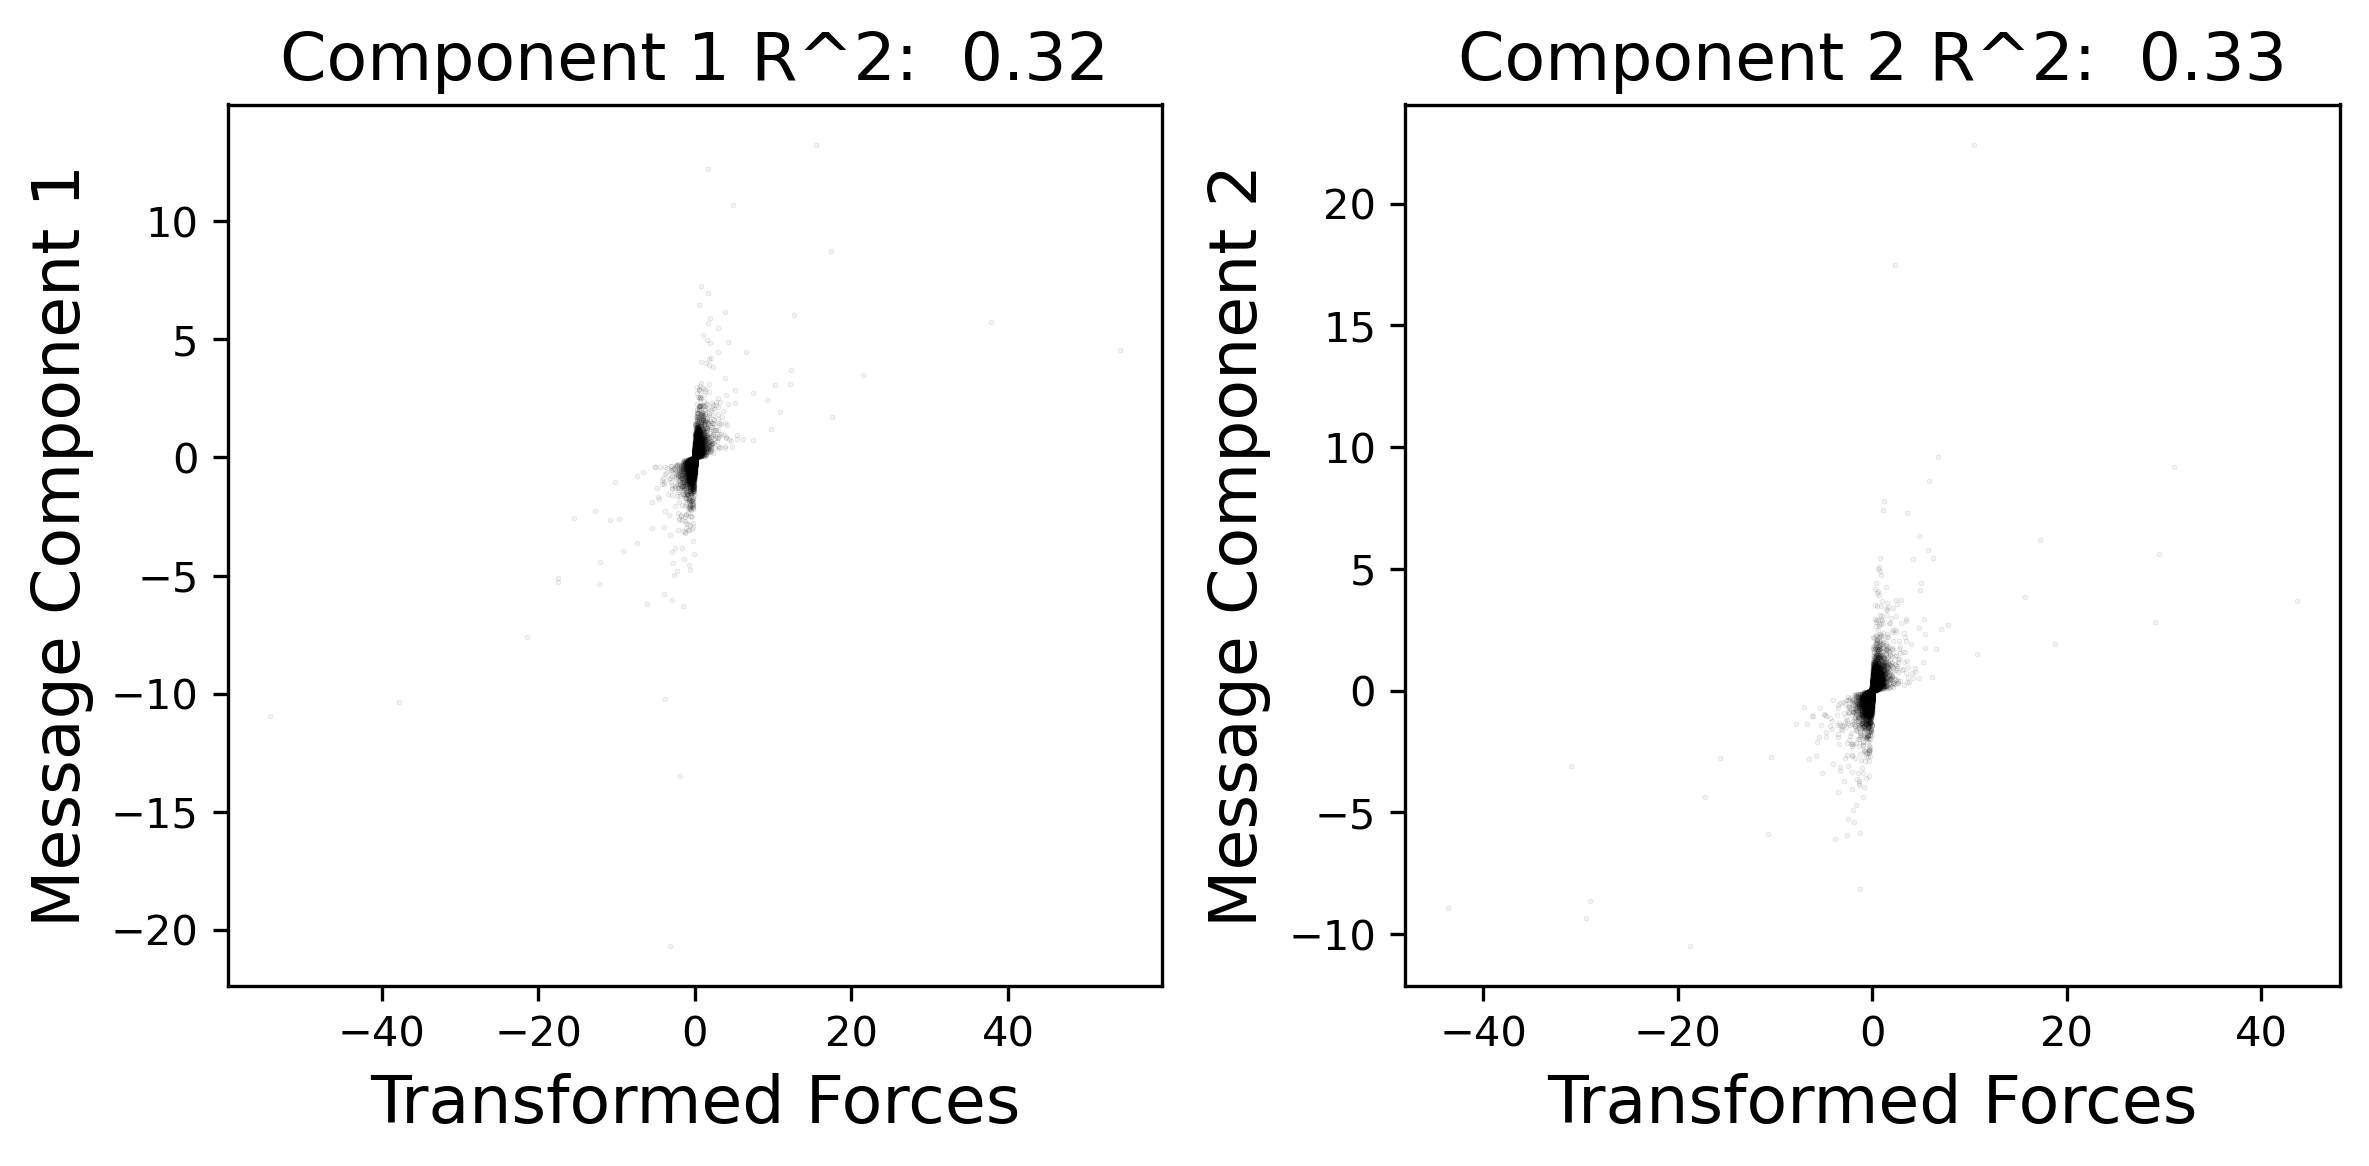
\includegraphics[width=\textwidth]{figs/r1_2d_force_r2.png}
        \caption{}
    \end{subfigure}
    \begin{subfigure}{0.45\textwidth}
        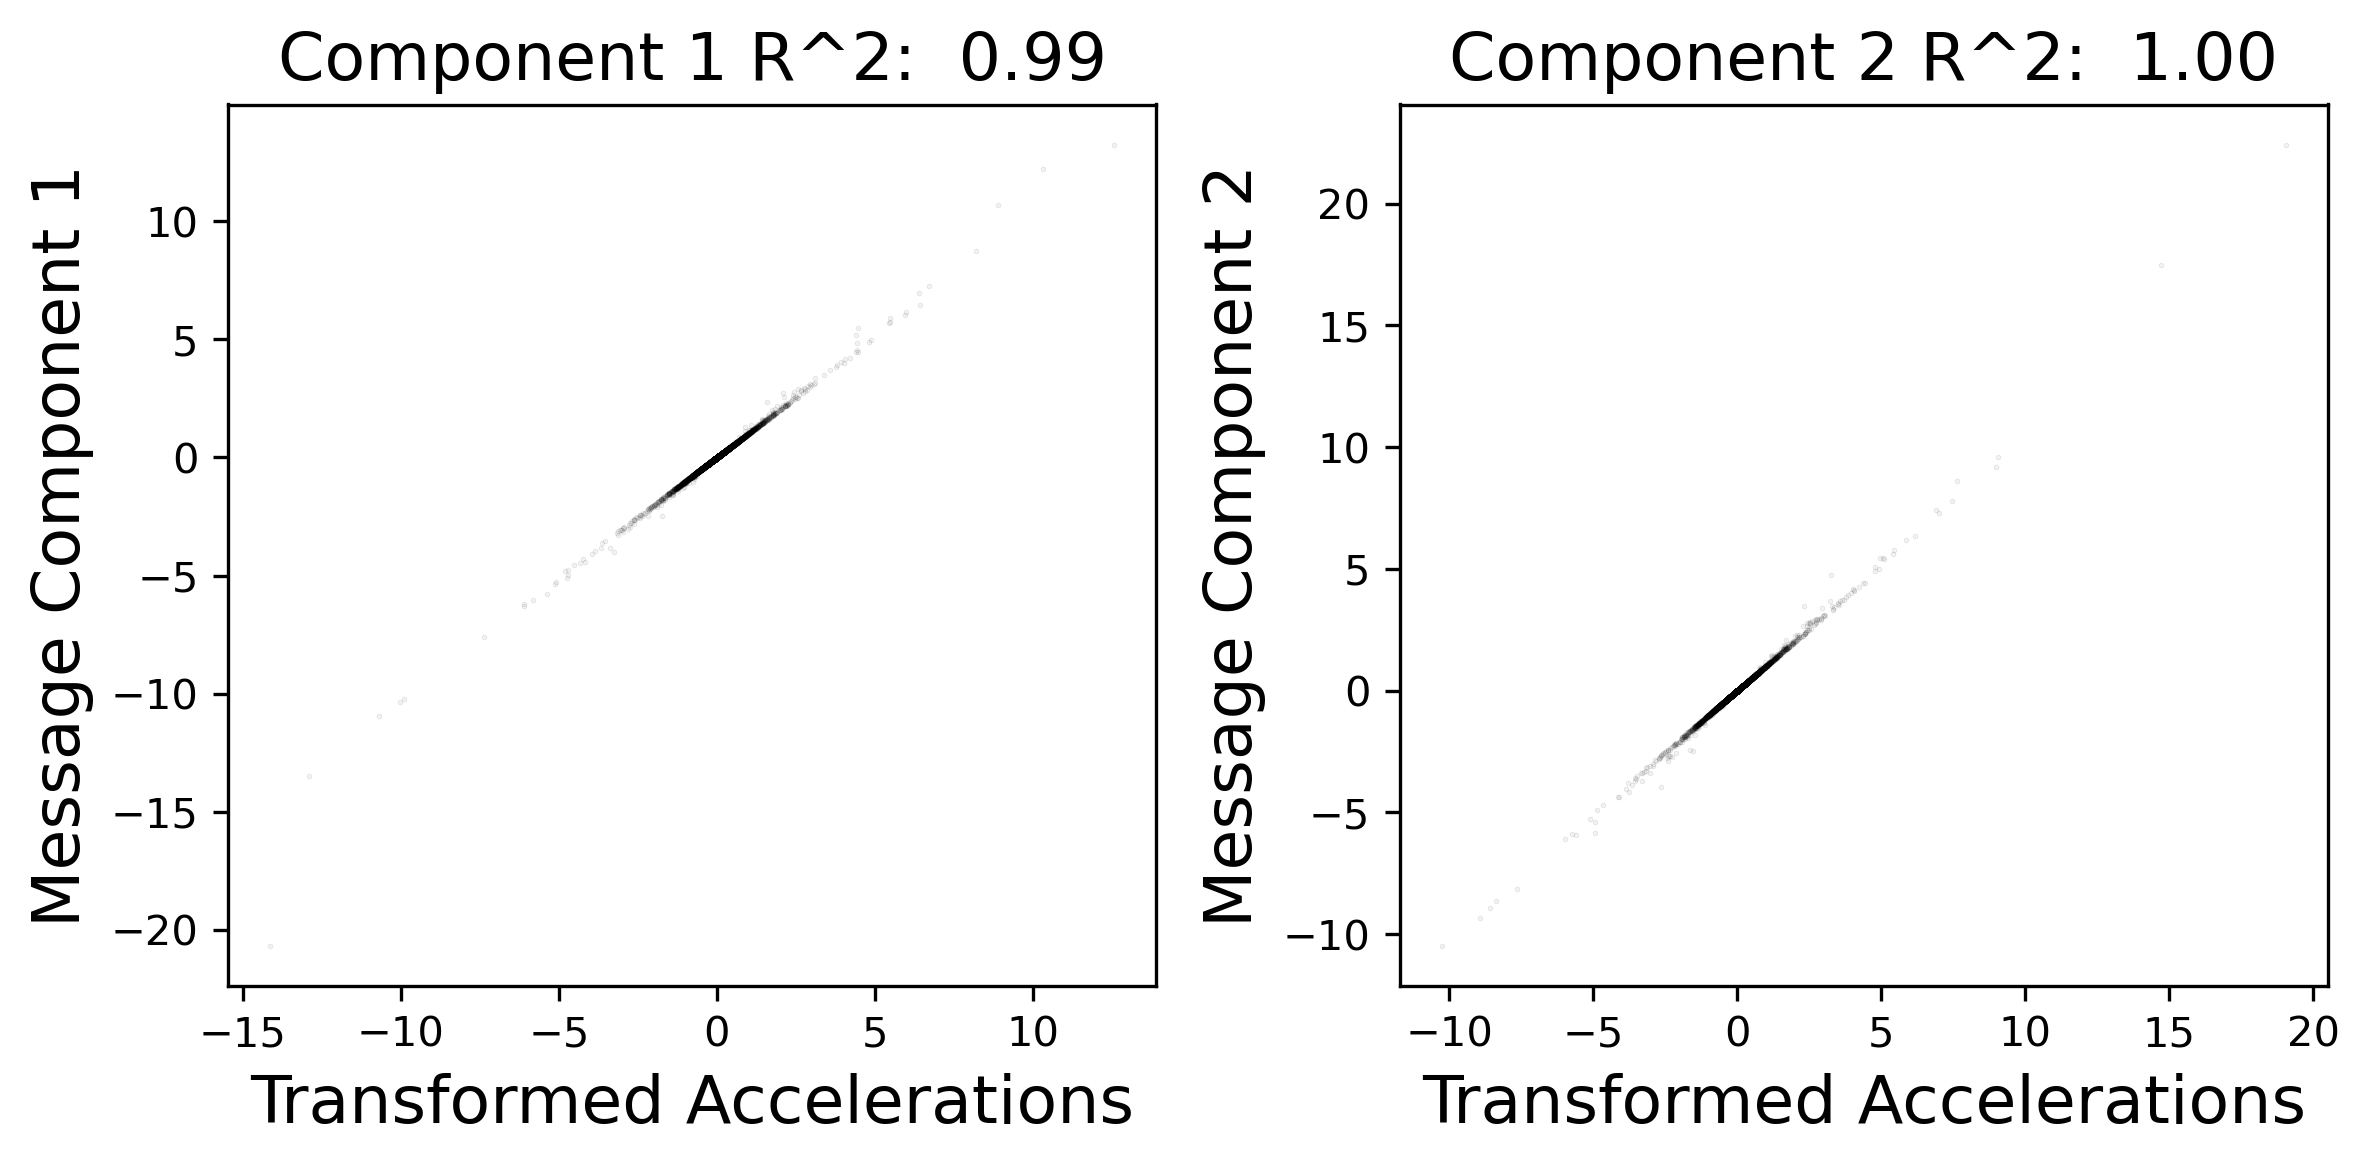
\includegraphics[width=\textwidth]{figs/r1_2d_accel_r2.png}
        \caption{}
    \end{subfigure}
    \caption{Comparison of scatter plots of the edge message components for $r^{-1}$ 2D, L1 experiment against a linear transformation of the a)  pairwise force b) pairwise acceleration.}
    \label{fig:scatter_plots}
\end{figure}
% Compare plot when
The subsequent results, as presented in Table \ref{tab:R2}, show that the pairwise force $R^2$ values for the bottleneck and L$_1$ strategies are significantly lower than the nearly perfect values reported in the original study. This discrepancy can be attributed to the edge model sometimes learning pairwise acceleration directly, rather than pairwise force. Indeed, this is also shown to be the case in the original paper where a successful reconstruction was shown for the $1/r^2$ bottleneck experiment where the edge model was distilled to give the pairwise acceleration. However, the impact of this was not commented on. Whether the edge model has learned the pairwise acceleration or force is a critical point to consider when interpreting the $R^2$ values that explicitly compare the edge message against the transformed force. For instance, Figure \ref{fig:scatter_plots} illustrates a scatter plot comparing the edge message components to a linear transformation of the true pairwise force versus pairwise acceleration for the model trained with the L1 regularisation strategy on the r$^{-1}$ 2D dataset, highlighting how the low $R^2$ values could be misleading. As such, in this report, two values are quoted for the $R^2$ metric, one for the pairwise force and one for the pairwise acceleration. When one is low, it is normally the case that the other is high. The next point to discuss is how contrary to the original paper, which suggests the standard strategy yields almost zero $R^2$ values, the findings in this report do not support this claim. The original paper also states that no model trained using the standard training strategy was found to give a successful reconstruction, indicating that a separate issue might be at play. The differences likely stem from variations in the datasets used, as discussed earlier. To investigate this, different seeds could be used to generate multiple datasets and this analysis could be repeated. 

% Sparsity in edge message not signficantly correlated with higher chance of symbolic reconstrucion, eg KL having sparser messages than L1 but being worse in the symbolic reconstruction. 
\subsection{Edge Message Sparsity}
The next set of results to be discussed are the sparsity values presented in the \ref{tab:scarcity}. While the original paper did not have any direct results which directly quantified the sparsity of the edge messages, the general argument was that sparsity in the edge message would lead to a greater probability of successful symbolic reconstructions. However, the findings for KL training strategy provide an interesting example where the edge messages were often found to be sparser than those coming from networks trained under the L$_{1}$ strategy, however it was the strategy which had the lowest number of successful symbolic reconstructions and worst test set MAE values. It is possible that the inductive bias placed on the model by the KL strategy was simply not appropriate for the task at hand. Alternatively, it may also be a case whereby the weight of the regularisation term was too large. In the original paper, the weight used for the KL divergence term was 1, compared to 0.01 for the L$_{1}$ strategy. It would be interesting to see how the performance of the KL strategy compared with the others with a smaller weight on the KL divergence term. In this case the solution might have simply over prioritised sparsity in the edge message over learning a good model, due to the weight, as opposed to something fundamentally wrong with the strategy. 
% Rough argument, kL had 99% of the variance captured in the first 2 components of its edge message however failed to reconstruct. Same for bottleneck. Sparsity at all costs not the best, as evidenced by the MAE performance of the strategy. 
\subsection{Symbolic Reconstructions}
% Discuss the edge reconstruction results - bottleneck wins, followed by l1, then standard and KL. 

Finally, the symbolic reconstructions are discussed. First the edge model reconstructions are considered. Similar to the original paper, the bottleneck strategy was the most successful strategy, having the highest number of successful reconstructions of the true pairwise force (or acceleration). This was followed by L1, standard and KL. It is no suprise that the bottleneck strategy is the most successful, as it places the strongest inductive bias on the model which explicitly constrains the latent space to be of the correct dimensionality. What is suprising however, is that the standard model performed much better than in the original paper, which found that no model trained under the standard strategy gave a successful reconstruction. In this reproduction, it was found that the standard strategy was able to give some successful reconstructions, despite not having any strategy to promote sparsity in the edge messages. It appears as though the inductive bias placed by using a message passing type network which predicts the acceleration from summed messages is already guides the model to learn a compact latent space more than was suggested by the results of the original paper.
% Explain why R2 is more useful metric to determine which experiments were successful.

To frame this discussion, it is important to make the point that to understand which strategy was successful in learning a representation that yielded the true pairwise force or acceleration, the appropriate table to consult is actually the $R^2$ Table \ref{tab:R2}. An $R^2$ value close to 1 is a sufficient condition to say that there exists a linear transformation of the true pairwise force or acceleration which strongly correlates with the significant edge message components. Such a linear transform can be reverse engineered to retrieve the symbolic model that best represents the edge model. 
% Explain why this is a rare situation whereby we know what to expect and why - why do we know that the edge model should be a linear transform of the true force / acceleration? - describe the linear latent space situation. 
------------------------------
TODO: Link in why we know the linear transform is best, what does this come from and how does this change for other experiments, why would we expect a linear relationship???

------------------------------------------------------
Therefore, the $R^2$ values can be used as a proxy to determine which training strategies were successful, which show that the standard, bottleneck and L1 strategies should all have more successful reconstructions. The issue with retrieving a symbolic model is that the search space is vast, despite using a subset of the operators considered in the original paper to reduce the search space. For example, the spring 3d bottleneck provides a good example of this point. Since it had an $R^2$ value close to 1, it was assumed that the model had learned an appropriate representation of the pairwise force. However, the symbolic search was unable to find a successful reconstruction. It took several attempts before a search yielded components that were close to the true pairwise force. Other experiments such as the spring 2D, spring 3D and $r^-1$ 2D and standard experiments all have $R^2$ values close to 1, however the single search performed was unable to find a successful reconstruction. It is very likely that if a longer search was done, as was the case for the spring 3D bottleneck experiment, a successful reconstruction would have been found. Therefore, the reconstructions presented should not be used as an absolute measure of the success of the training strategy, but rather as a guide to determine which strategies are more likely to have been successful. 
% However it still is not somewhat necessary - original paper claims an R2 of 0.2 for KL yet a succesful reconstruction was found, this is confusing 
It is also important to note that while it is not strictly necessary that the experiment have a high $R^2$ value in order for symbolic regression to be successful, it is also the case that one would expect the $R^2$ value to indicate moderate correlation if the symbolic regression was successful. However, the original paper presents conflicting results for the KL strategy, where the spring and $r^{-1}$ 3D experiments had $R^2$ values of was 0.214 and 0.332, respectively, yet both were stated to give successful reconstructions. Such a discrepancy is confusing and should be investigated further. 
% Discuss the results of the node model - l1  wins, followed by standard, bottleneck and KL.

Next the node model results are discussed. The results show that the L1 and standard strategues performed the best, followed by bottleneck and with doing much worst than the others KL. Future work could include creating $R^2$ tables for the node model to better understand if reconstructions were missed as discussed earlier or if the experiments were truly unsuccessful. This could be done by finding the correlation between the node model outputs and a linear transform of the aggregated edge message and node features in the same way as was done for the edge model.


It is worth noting that many reconstructions were very close to the correct one, however were excluded as it was not clear how strict the original paper was when approving a given reconstruction as successful. Some examples of close reconstructions are given in the appendix. Further, sometimes the correct reconstruction was not the best, where best is defined by the selection criteria outlined in the method. Therefore, these results are an underestimate of the true number of successful reconstructions. Finally, only 1000 samples were used to perform the reconstructions, whereas the original paper used 5000. Using more samples would likely lead to more successful reconstructions, however the analysis would take much longer and so was not done in this report as for most experiments, 1000 samples was sufficient to find a successful reconstruction.

The final set of results to discuss are those from comparing the symbolic model's performance to the trained networks. The results show that the symbolic model outperforms the neural network for the spring 2D simulation and is comparable with the neural network for the r$^{-1}$ 2D simulation. For the remaining simulations, the neural network significantly outperforms the symbolic model. It is worth noting that the constants in the symbolic model were not refit to the data as suggested in the original paper. This could be a reason for the poor performance of the symbolic model in the other simulations. It would be interesting to see how the symbolic model would perform if the constants were refit to the data. Given that there is no noise in the dataset, one would expect the symbolic model to perform at least as well as the neural network, if not better. It is likely performing worse due to the accumulated approximation error from the multiple levels of function fitting.
% Performs increasingly worse as the force law becomes more complex, likely due to the learnt constants being incorrect, would be interesting to see the effect of refitting the constants.

% Interesting artifact whereby node model undid error in the edge model and in composition the model was correct.
\subsection{Future work}
    % Dataset reproduction being very hard.
    There are two primary means by which this reproduction study could be further improved. The first being to repeat the analysis for different random seeds and seeing if the different sets of trained models are consistent with the results presented in this report. This would help give an understanding of what is natural variation in the results due to the stochastic nature of the training process versus what is a systematic discrepancy between the reproduced study and the original findings. Such an approach would solidify the conclusions drawn and provide a clearer comparison between the varying strategies employed for both the edge and node models.

    The second means by which this reproduction study could be further improved is to investigate the effect incorporating more inductive biases and seeing if the trained models are easier to distill as would be expected. A natural bias to add to the model would be to include newtons third law, through introducing a penalty to the loss term that enforces the sum of $\mathbf{\phi^{e}(x_i, x_j)} + \mathbf{\phi^e(x_j,x_i)} = \textbf{0}$.

\section{ Reproducibility}
This section addresses the reproducibility aspect of this work. There are 3 sources of randomness at play which affect the ability to reproduce the results. 
\subsection{Dataset Reproducability}
The first challenge reproducing the results of the original paper was in reproducing the datasets. The original paper did provide the code used to generate the datasets, however did not indicate which seeds were used. However even if this was declared, it is likely that the datasets would still be difficult to reproduce, due to the differences in hardware. $N$ body simulations, where $N > 2$, are famously chaotic systems. This means that small changes in the initial conditions can lead to vastly different outcomes. Or in this case, small numerical fluctuations introduced through the hardware specific optimisations that the \texttt{jax} package uses can lead to drastically different trajectories. To demonstrate this point, two datasets are generated following the $r^{-1}$ force law, for 4 bodies in 2 dimensions. The dataset describes 10000 simulations of 30 time steps each. The same random seed was used to generate both datasets, however the datasets were generated on different machines, the first was generated locally on a laptop using macOS and the second was generated through a system running linux. The Kologorov-Smirnov test was used to compare the distributions of the particles $x$ coordinate as a function of time across all simulations. The results are shown in Figure \ref{fig:ks_test}. The figure shows how the p value rapidly decreases as the time step increases, indicating that the distributions quickly diverge. 

\begin{figure}[H]
    \centering
    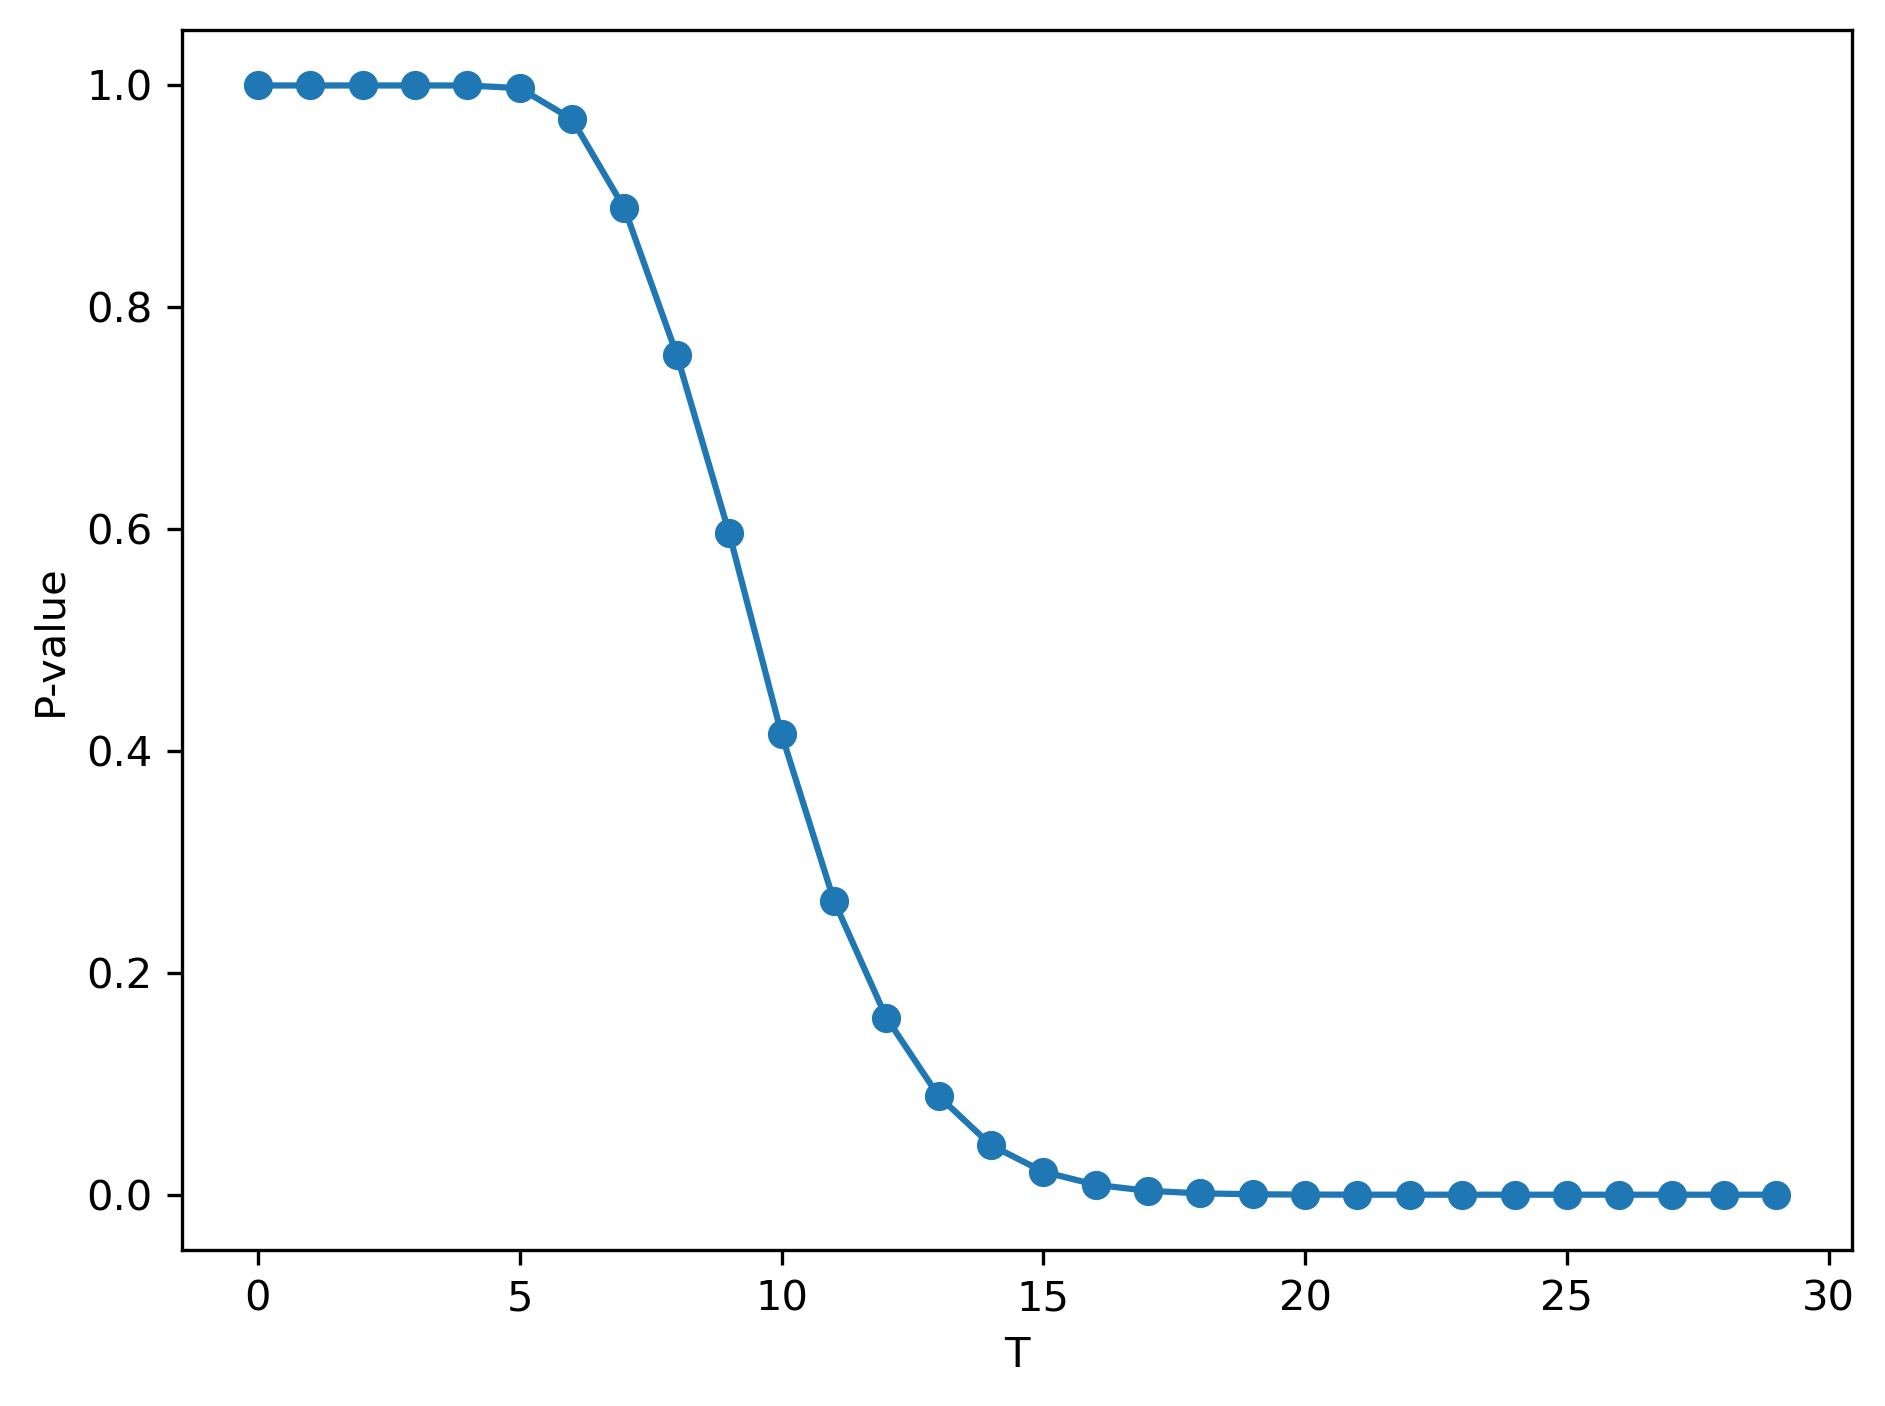
\includegraphics[width=0.5\textwidth]{figs/ks_test.png}
    \caption{Kologorov-Smirnov test comparing the distributions of the particles $x$ coordinate as a function of time, $T$ across an interacting particle dataset. The test was performed on two datasets generated using the same package versions and random seeds but on two different machines.}
    \label{fig:ks_test}
\end{figure}
Thus, to address this issue, the datasets were generated using a docker container. This ensures a standardised environment in which to generate the datasets in a reproducible manner. Further, future work could instead incorporate datasets which use more simulations that are each evolved for fewer number of time steps which would help limit any error introduced by the chaotic nature of the system. Alternatively, the datasets could be hosted on a cloud service, such as AWS S3, which would circumvent the need to generate the datasets and guarentee that everyone is using the same data.

\subsection{Model Reproducability}
Next, even if the datasets can be perfectly reproduced, there are still stochastic elements in the training process which can affect the results. To resolve this, a random seed was used to make training deterministic and see the initial model weights are also saved during training. These can be made available upon request. Further, the code base was designed to give reproducible results. Conda was used to standardise the environment and configuration files used to run the experiments were stored in the git repository under \texttt{configs/train\_configs}. Every train job is automatically logged to wandb. The train config is also saved to the output directory of the train job with the current git commit hash. These configs and the trained models can be made available upon request, they have not been included in the git repository due to their size. Steps to reproduce the training process are detailed in the \texttt{README.md} file.

\subsection{Symbolic Regression Reproducbility}
Lastly, the symbolic regression process is also stochastic. The search space is vast and thus in order to get reproducible results, a random state was set. Further, the hyperparameters of the \texttt{PySRRegressor} were also made clear in the method section.

% 3 sources of randomness - the dataset , model initialisation, optimisation / training, symbolic search. How to standardise each one in the future.

% Dockerisation, conda, git, readme, etc.

\section{Conclusion}
This report has presented the results of a reproduction study of the paper "Discovering Symbolic Models using Deep Learning with Inductive Biases". Here a subset of the experiments introduced in the original paper were investigated. This report managed to find the same overall trends in the MAE values as the original paper, however the MAE values were consistently lower due to the extra preprocessing step of pruning the data. Symbolic reconstructions of the edge and node models were successfully found. With the bottleneck and L1 training strategies being the most successful in yielding the most reconstructions of the true force law. The standard strategy was found to be far more successful in learning a compact latent space than was suggested by the original paper. The symbolic model was compared against the neural network model and found to perform better for the spring 2D simulation and comparable for the r$^{-1}$ 2D simulation. Thus, the main claim of the original paper, that symbolic regression can be used to distill the learned models of neural networks trained using appropriate inductive biases, was found to be true. 
%     Talk about perhaps the more sensible thing would be to distill one at a time in accordance with the framework.
%     Effect of training for fewer epochs
%     Discuss challenges reproducing the results of the paper.
%     Discuss how the code base is designed to give reproduible results
%     Dataset storage.
%     Dataset seed and local environment differences.
%     Try to generate the dataset from a docker container to standardise the environment.
%     Config files git commits, wandb
%     Future work, squash velocity, use a larger eps and see if the model can learn this, squash the log var. For data pre processing 
%     Preprocessing not in paper but got nans in kl otherwise
%     Explore purely velocity based pre pru
%     , NL3, enforcing correctness of dimensional units.
%     Discussion point - stronger L1 or an L1 scheduler type thing.
%     Could make the data more reproducable by fewer time steps and more simulations
    
    
    
    
    
    
    
    
    \section{Appendix}
    Example of a failed reconstruction:
    Spring 3D, $L_1$: expect $\phi^{e}_i \approx (1-\frac{1}{r})\mathbf{a} \cdot \mathbf{\Delta r} + b$.
    
    $$\phi^{e}_1 = (0.0772r + 0.102)(0.381 \Delta x - 0.190 \Delta y + \Delta z)$$

    Example of close reconstructions but 2nd was good.

    Example of undoing reconstruction.

    Dump of the histograms of the pruning.

    

\bibliographystyle{plain}  % Choose the style that suits your needs
\bibliography{references}  
\end{document}

